\question
Which of the following functions is continuous at $x=0$ ?
\begin{choices}
  \choice $f(x) \begin{cases}\sin \dfrac{1}{x} & \text { for } x \neq 0 \\ 0 & \text { for } x=0\end{cases}$
  \choice $f(x)=[x]$ (greatest-integer function)
  \choice $f(x) \begin{cases}\dfrac{x}{x} & \text { for } x \neq 0 \\ 0 & \text { for } x=0\end{cases}$
  \CorrectChoice $f(x) \begin{cases}x \sin \dfrac{1}{x} & \text { for } x \neq 0 \\ 0 & \text { for } x=0\end{cases}$
  \choice $f(x)=\dfrac{x+1}{x}$
\end{choices}
\begin{solution}
If $f(x)=x \sin \dfrac{1}{x}$ for $x \neq 0$ and $f(0)$, then


\[
\lim\limits_{x \to 0} f(x)=0=f(0) ;
\]

thus this function is continuous at 0 . In (A), $\lim\limits_{x \to 0} \sin \dfrac{1}{x}$ does not exist; in (B), $f$ has a jump discontinuity; in (C), $f$ has a removable discontinuity; and in (E), $f$ has a removable discontinuity.
\end{solution}

\question
Which of the following statements about the graph of $y=\dfrac{x^{2}+1}{x^{2}-1}$ is not true?
\begin{choices}
  \choice The graph is symmetric to the $y$-axis.
  \choice The graph has two vertical asymptotes.
  \CorrectChoice There is no $y$-intercept.
  \choice The graph has one horizontal asymptote.
  \choice There is no $x$-intercept.
\end{choices}
\begin{solution}
(C) To find the $y$-intercept, let $x=0 ; y=-1$.
\end{solution}

\question
$\lim\limits_{x \to 1^{-}}([x]-|x|)=$
\begin{choices}
  \CorrectChoice $-1$
  \choice $0$
  \choice $1$
  \choice $2$
  \choice none of these
\end{choices}
\begin{solution}
(A) $\lim\limits_{x \to 1^{-}}[x]-\lim\limits_{x \to 1^{-}}|x|=0-1=-1$.
\end{solution}




\newpage




\question
The $x$-coordinate of the point on the curve $y=x^{2}-2 x+3$ at which the tangent is perpendicular to the line $x+3 y+3=0$ is
\begin{choices}
  \choice $-\dfrac{5}{2}$
  \choice $-\dfrac{1}{2}$
  \choice $\dfrac{7}{6}$
  \CorrectChoice $\dfrac{5}{2}$
  \choice none of these
\end{choices}
\begin{solution}
(D) The line $x+3 y+3=0$ has slope $-\dfrac{1}{3}$; a line perpendicular to it has slope 3 .

The slope of the tangent to $y=x^{2}-2 x+3$ at any point is the derivative $2 x-2$. Set $2 x-2$ equal to 3 .
\end{solution}

\question
$\lim\limits_{x \to 1} \dfrac{\dfrac{3}{x}-3}{x-1}$ is
\begin{choices}
  \CorrectChoice $-3$
  \choice $-1$
  \choice $1$
  \choice $3$
  \choice nonexistent
\end{choices}
\begin{solution}
(A) $\lim\limits_{x \to 1} \dfrac{\dfrac{3}{x}-3}{x-1}$ is $f^{\prime}(1)$, where $f(x)=\dfrac{3}{x}, f^{\prime}(x)=-\dfrac{3}{x^{2}}$. Or simplify the given\\
fraction to $\dfrac{3-3 x}{x(x-1)}=\dfrac{3(1-x)}{x(x-1)}=\dfrac{-3}{x}(x \neq 1)$.
\end{solution}

\question
$\ln \left(3 e^{x+2}\right)-\ln \left(3 e^{x}\right)=$
\begin{choices}
  \CorrectChoice $2$
  \choice $e^{2}$
  \choice $2 \ln 3$
  \choice $\ln 3+2$
  \choice $2 \ln 3+2$
\end{choices}
\begin{solution}
(A) $\ln \left(3 e^{x+2}\right)-\ln \left(3 e^{x}\right)=\ln \dfrac{3 e^{x+2}}{3 e^{x}}=\ln e^{2}=2 \ln e=2$.
\end{solution}
 

\newpage

\question
$\displaystyle\int_{0}^{6}|x-4| d x=$
\begin{choices}
  \choice $6$
  \choice $8$
  \CorrectChoice $10$
  \choice $11$
  \choice $12$
\end{choices}
\begin{solution}
(C) $\displaystyle\int_{0}^{6}|x-4| d x=\displaystyle\int_{0}^{4}(4-x) d x+\displaystyle\int_{4}^{6}(x-4) d x=\left.\left(4 x-\dfrac{x^{2}}{2}\right)\right|_{0} ^{4}+\left.\left(\dfrac{x^{2}}{2}-4 x\right)\right|_{4} ^{6}$

\[
=8+[(18-24)-(8-16)]=8+(-6+8)=10 .
\]

Save time by finding the area under $y=|x-4|$ from a sketch!\\
\begin{center}
  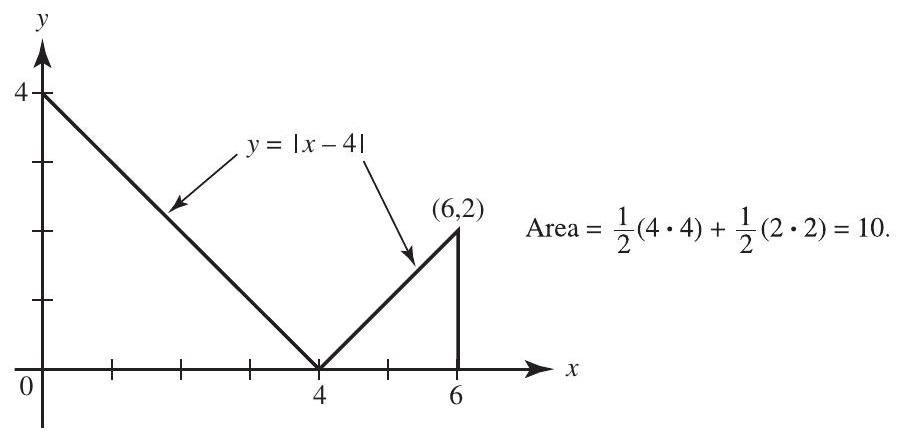
\includegraphics[width=0.70\linewidth]{calculus/images/4dd0024d-5e0f-40f8-af74-ec664288d8ef-19_440_898_1066_640.jpg}
\end{center}
\end{solution}

\question
$\lim\limits_{x \to \infty} \dfrac{3+x-2 x^{2}}{4 x^{2}+9}$ is
\begin{choices}
  \CorrectChoice $-\dfrac{1}{2}$
  \choice $\dfrac{1}{2}$
  \choice $1$
  \choice $3$
  \choice nonexistent
\end{choices}
\begin{solution}
(A) Since the degrees of numerator and denominator are the same, the limit as $x \to \infty$ is the ratio of the coefficients of the terms of highest degree: $\dfrac{-2}{4}$.
\end{solution}



\newpage




\question
The maximum value of the function $f(x)=x^{4}-4 x^{3}+6$ on the closed interval $[1,4]$ is
\begin{choices}
  \choice $1$
  \choice $0$
  \choice $3$
  \CorrectChoice $6$
  \choice none of these
\end{choices}
\begin{solution}
(D) On the interval $[1,4], f^{\prime}(x)=0$ only for $x=3$. Since $f$ (3) is a relative minimum, check the endpoints to find that $f(4)=6$ is the absolute maximum of the function.
\end{solution}

\question
Let $\left\{\begin{array}{l}f(x)=\dfrac{\sqrt{x+4}-3}{x-5} \text { if } x \neq 5 \text {, and let } f \text { be continuous at } x=5 \text {. Then } c= \\ f(5)=c\end{array}\right.$
\begin{choices}
  \choice $-\dfrac{1}{6}$
  \choice $0$
  \CorrectChoice $\dfrac{1}{6}$
  \choice $1$
  \choice $6$
\end{choices}
\begin{solution}
(C) To find $\lim f$ as $x \to 5$ (if it exists), multiply $f$ by $\dfrac{\sqrt{x+4}+3}{\sqrt{x+4}+3}$.

\[
f(x)=\dfrac{x-5}{(x-5)(\sqrt{x+4}+3)}
\]

and if $x \neq 5$ this equals $\dfrac{1}{\sqrt{x+4}+3}$. So $\lim f(x)$ as $x \to 5$ is $\dfrac{1}{6}$. For $f$ to be continuous at $x=5, f(5)$ or $c$ must also equal $\dfrac{1}{6}$.
\end{solution}

\question
$\displaystyle\int_{0}^{\pi / 2} \cos ^{2} x \sin x d x=$
\begin{choices}
  \choice $-1$
  \choice $-\dfrac{1}{3}$
  \choice $0$
  \CorrectChoice $\dfrac{1}{3}$
  \choice $1$
\end{choices}
\begin{solution}
(D) Evaluate $-\left.\dfrac{1}{3} \cos ^{3} x\right|_{0} ^{\pi / 2}$.
\end{solution}




\newpage




\question
If $\sin x=\ln y$ and $0<x<\pi$, then, in terms of $x, \dfrac{d y}{d x}$ equals
\begin{choices}
  \CorrectChoice $e^{\sin x} \cos x$
  \choice $e^{-\sin x} \cos x$
  \choice $\dfrac{e^{\sin x}}{\cos x}$
  \choice $e^{\cos x}$
  \choice $e^{\sin x}$
\end{choices}
\begin{solution}
(A) $\cos x=\dfrac{1}{y} \dfrac{d y}{d x}$ and thus $\dfrac{d y}{d x}=y \cos x$. From the equation given, $y=e^{\sin x}$.
\end{solution}

\question
If $f(x)=x \cos x$, then $f^{\prime}\left(\dfrac{\pi}{2}\right)$ equals
\begin{choices}
  \choice $\dfrac{\pi}{2}$
  \choice $0$
  \choice $-1$
  \CorrectChoice $-\dfrac{\pi}{2}$
  \choice $1$
\end{choices}
\begin{solution}
(D) If $f(x)=x \cos x$, then $f^{\prime}(x)=-x \sin x+\cos x$, and

\[
f^{\prime}\left(\dfrac{\pi}{2}\right)=-\dfrac{\pi}{2} \cdot 1+0
\]


\end{solution}

\question
The equation of the tangent to the curve $y=e^{x} \ln x$, where $x=1$, is
\begin{choices}
  \choice $y=e x$
  \choice $y=e^{x}+1$
  \CorrectChoice $y=e(x-1)$
  \choice $y=e x+1$
  \choice $y=x-1$
\end{choices}
\begin{solution}
If $y=e^{x} \ln x$, then $\dfrac{d y}{d x}=\dfrac{e^{x}}{x}+e^{x} \ln x$, which equals $e$ when $x=1$. Since also $y=0$ when $x=1$, the equation of the tangent is $y=e(x-1)$.
\end{solution}




\newpage




\question
If the displacement from the origin of a particle moving along the $x$-axis is given by $s=3+(t-2)^{4}$, then the number of times the particle reverses direction is
\begin{choices}
  \choice $0$
  \CorrectChoice $1$
  \choice $2$
  \choice $3$
  \choice none of these
\end{choices}
\begin{solution}
$v=4(t-2)^{3}$ and changes sign exactly once, when $t=2$.
\end{solution}

\question
$\displaystyle\int_{-1}^{0} e^{-x} d x$ equals
\begin{choices}
  \choice $1-e$
  \choice $\dfrac{1-e}{e}$
  \CorrectChoice $e-1$
  \choice $1-\dfrac{1}{e}$
  \choice $e+1$
\end{choices}
\begin{solution}
Evaluate $-\left.e^{-x}\right|_{-1} ^{0}$.
\end{solution}

\question
If $f(x)=\left\{\begin{array}{lr}x^{2} & \text { for } x \leq 2 \\ 4 x-x^{2} & \text { for } x>2\end{array}\right.$, then $\displaystyle\int_{-1}^{4} f(x) d x$ equals
\begin{choices}
  \choice $7$
  \choice $\dfrac{23}{3}$
  \CorrectChoice $\dfrac{25}{3}$
  \choice $9$
  \choice $\dfrac{65}{3}$
\end{choices}
\begin{solution}
$\displaystyle\int_{-1}^{4} f(x) d x=\displaystyle\int_{-1}^{2} x^{2} d x+\displaystyle\int_{2}^{4}\left(4 x-x^{2}\right) d x=\left.\dfrac{x^{3}}{3}\right|_{-1} ^{2}+\left.\left(2 x^{2}-\dfrac{x^{3}}{3}\right)\right|_{2} ^{4}$.
\end{solution}




\newpage




\question
If the position of a particle on a line at time $t$ is given by $s=t^{3}+3 t$, then the speed of the particle is decreasing when
\begin{choices}
  \choice $-1<t<1$
  \choice $-1<t<0$
  \CorrectChoice $t<0$
  \choice $t>0$
  \choice $|t|>1$
\end{choices}
\begin{solution}
Since $v=3 t^{2}+3$, it is always positive, while $a=6 t$ and is positive for $t>0$ but negative for $t<0$. The speed therefore increases for $t>0$ but decreases for $t<0$.
\end{solution}

\question
A rectangle with one side on the $x$-axis is inscribed in the triangle formed by the lines $y=x, y=0$, and $2 x+y=12$. The area of the largest such rectangle is
\begin{choices}
  \CorrectChoice $6$
  \choice $3$
  \choice $\dfrac{5}{2}$
  \choice $5$
  \choice $7$
\end{choices}
\begin{solution}
Note from the figure that the area, $A$, of a typical rectangle is
\[
A=\left(x_{2}-x_{1}\right) \cdot y=\left(\dfrac{12-y}{2}-y\right) \cdot y=6 y-\dfrac{3 y^{2}}{2} .
\]
\begin{center}
  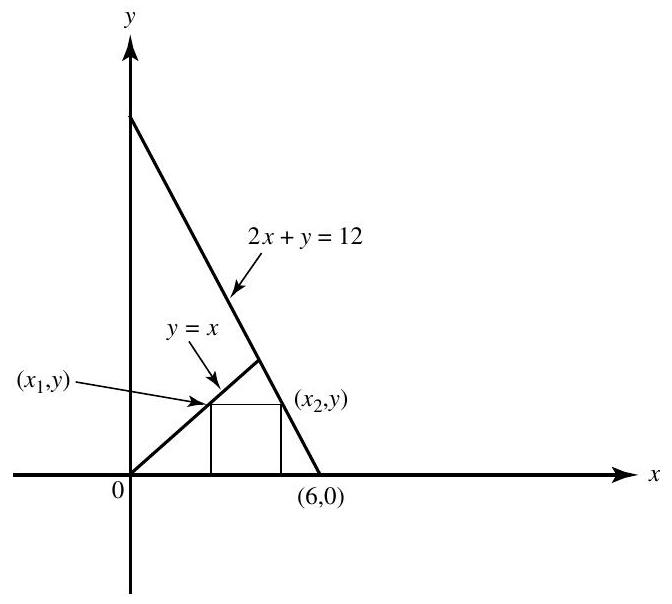
\includegraphics[width=0.40\linewidth]{calculus/images/4dd0024d-5e0f-40f8-af74-ec664288d8ef-20_604_672_1491_1124.jpg}
\end{center}
For $y=2, \dfrac{d A}{d y}=0$. Note that $\dfrac{d^{2} A}{d y^{2}}$ is always negative.
\end{solution}




\newpage




\question
The abscissa of the first-quadrant point that is on the curve of $x^{2}-y^{2}=1$ and closest to the point $(3,0)$ is
\begin{choices}
  \choice $1$
  \CorrectChoice $\dfrac{3}{2}$
  \choice $2$
  \choice $3$
  \choice none of these
\end{choices}
\begin{solution}
(B) If $S$ represents the square of the distance from $(3,0)$ to a point $(x, y)$ on the curve, then $S=(3-x)^{2}+y^{2}=(3-x)^{2}+\left(x^{2}-1\right)$. Setting $\dfrac{d S}{d x}=0$ yields the minimum distance at $x=\dfrac{3}{2}$.
\end{solution}

\question
If $y=\ln (4 x+1)$, then $\dfrac{d^{2} y}{d x^{2}}$ is
\begin{choices}
  \choice $\dfrac{1}{4}$
  \choice $\dfrac{-1}{(4 x+1)^{2}}$
  \choice $\dfrac{-4}{(4 x+1)^{2}}$
  \CorrectChoice $\dfrac{-16}{(4 x+1)^{2}}$
  \choice $\dfrac{-1}{16(4 x+1)^{2}}$
\end{choices}
\begin{solution}
(D) $\dfrac{d y}{d x}=\dfrac{4}{4 x+1}=4(4 x+1)^{-1}$, so $\dfrac{d^{2} y}{d x^{2}}=4\left(-1(4 x+1)^{-2} \cdot 4\right)$
\end{solution}



\newpage



\question
The region bounded by the parabolas $y=x^{2}$ and $y=6 x-x^{2}$ is rotated about the $x$-axis so that a vertical line segment cut off by the curves generates a ring. The value of $x$ for which the ring of largest area is obtained is
\begin{choices}
  \choice $4$
  \choice $3$
  \choice $\dfrac{5}{2}$
  \CorrectChoice $2$
  \choice $\dfrac{3}{2}$
\end{choices}
\begin{solution}
(D) See the figure. Since the area, $A$, of the ring equals $\pi\left(y_{2}{ }^{2}-y_{1}{ }^{2}\right)$,

\[
A=\pi\left[\left(6 x-x^{2}\right)^{2}-x^{4}\right]=\pi\left[36 x^{2}-12 x^{3}+x^{4}-x^{4}\right]
\]

and $\dfrac{d A}{d x}=\pi\left(72 x-36 x^{2}\right)=36 \pi x(2-x)$.\\
It can be verified that $x=2$ produces the maximum area.\\
\begin{center}
  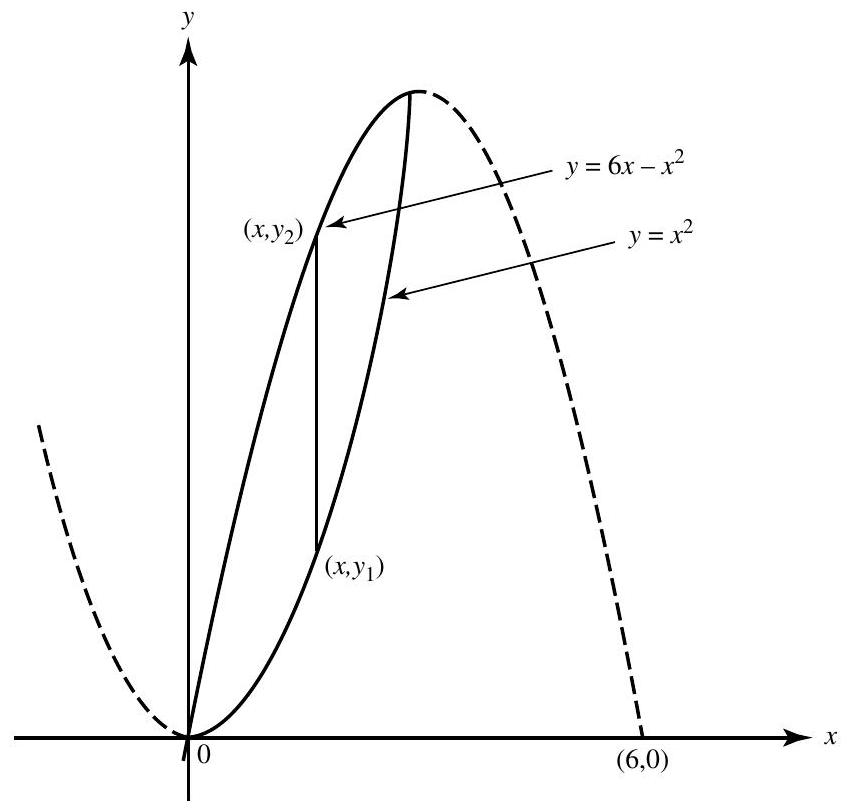
\includegraphics[width=0.40\linewidth]{calculus/images/4dd0024d-5e0f-40f8-af74-ec664288d8ef-21_811_848_797_663.jpg}
\end{center}
\end{solution}



\newpage



\question
$\int \dfrac{d x}{x \ln x}$ equals
\begin{choices}
  \CorrectChoice $\ln (\ln x)+C$
  \choice $-\dfrac{1}{\ln ^{2} x}+C$
  \choice $\dfrac{(\ln x)^{2}}{2}+C$
  \choice $\ln x+C$
  \choice none of these
\end{choices}
\begin{solution}
(A) This is of type $\int \dfrac{d u}{u}$ with $u=\ln x: \int \dfrac{\dfrac{1}{x} d x}{\ln x}$.\\
\begin{center}
  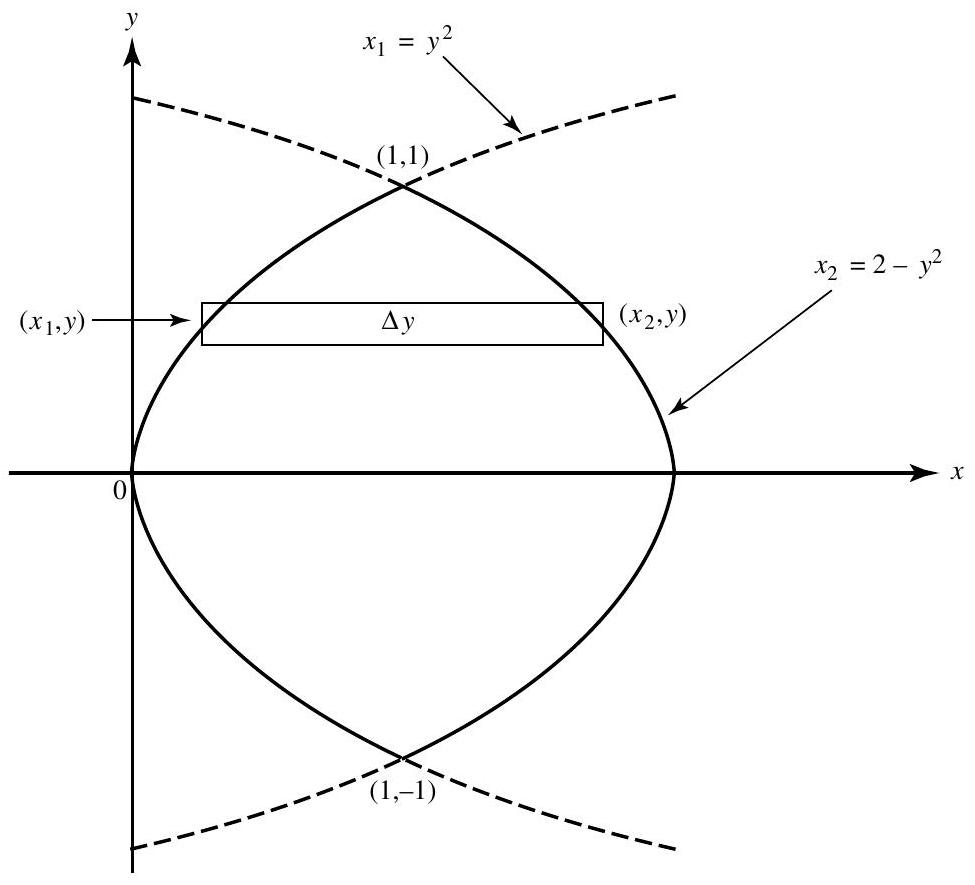
\includegraphics[width=0.40\linewidth]{calculus/images/4dd0024d-5e0f-40f8-af74-ec664288d8ef-21_885_975_1857_598.jpg}
\end{center}
\end{solution}

\question
The volume obtained by rotating the region bounded by $x=y^{2}$ and $x=2-y^{2}$ about the $y$-axis is equal to
\begin{choices}
  \CorrectChoice $\dfrac{16 \pi}{3}$
  \choice $\dfrac{32 \pi}{3}$
  \choice $\dfrac{32 \pi}{15}$
  \choice $\dfrac{64 \pi}{15}$
  \choice $\dfrac{8 \pi}{3}$
\end{choices}
\begin{solution}
(A) About the $y$-axis; see the figure. Washer.
\[
\Delta V=\pi\left(x_{2}^{2}-x_{1}^{2}\right) \Delta y, \text { so } V=2 \pi \displaystyle\int_{0}^{1}\left[\left(2-y^{2}\right)^{2}-y^{4}\right] d y=2 \pi \displaystyle\int_{0}^{1}\left(4-4 y^{2}\right) d y
\]
\end{solution}





\newpage





\question
The general solution of the differential equation $\dfrac{d y}{d x}=\dfrac{1-2 x}{y}$ is a family of
\begin{choices}
  \choice straight lines
  \choice circles
  \choice hyperbolas
  \choice parabolas
  \CorrectChoice ellipses
\end{choices}
\begin{solution}
Separating variables, we get $y d y=(1-2 x) d x$. Integrating gives
\[
\dfrac{1}{2} y^{2}=x-x^{2}+C
\]
or
\[
y^{2}=2 x-2 x^{2}+k
\]
or
\[
2 x^{2}+y^{2}-2 x=k .
\]
\end{solution}

\question
Estimate $\displaystyle\int_{0}^{4} \sqrt{25-x^{2}} d x$ using the Left Rectangular Rule and two subintervals of equal width.
\begin{choices}
  \choice $3+\sqrt{21}$
  \choice $5+\sqrt{21}$
  \choice $6+2 \sqrt{21}$
  \choice $8+2 \sqrt{21}$
  \CorrectChoice $10+2 \sqrt{21}$
\end{choices}
\begin{solution}
$2(5)+2 \sqrt{21}$.\\
\begin{center}
  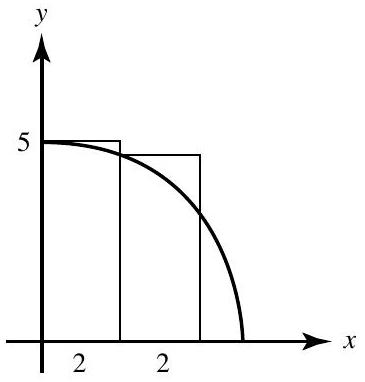
\includegraphics[width=0.40\linewidth]{calculus/images/4dd0024d-5e0f-40f8-af74-ec664288d8ef-22_382_365_1173_1060.jpg}
\end{center}
\end{solution}






\newpage





\question
$\displaystyle\int_{0}^{7} \sin \pi x d x=$
\begin{choices}
  \choice $-2$
  \choice $-\dfrac{2}{\pi}$
  \choice $0$
  \choice $\dfrac{1}{\pi}$
  \CorrectChoice $\dfrac{2}{\pi}$
\end{choices}
\begin{solution}
$\dfrac{1}{\pi} \displaystyle\int_{0}^{7} \sin \pi x(\pi d x)=\left.\dfrac{-1}{\pi} \cos (\pi x)\right|_{0} ^{7}$.
\end{solution}

\question
$\lim\limits_{x \to 0} \dfrac{\tan 3 x}{2 x}=$
\begin{choices}
  \choice $0$
  \choice $\dfrac{1}{2}$
  \choice $\dfrac{2}{3}$
  \CorrectChoice $\dfrac{3}{2}$
  \choice $\infty$
\end{choices}
\begin{solution}
Use L'Hpital's Rule or rewrite the expression as $\lim\limits_{x \to \infty} \dfrac{\sin 3 x}{3 x} \cdot \dfrac{1}{\cos 3 x} \cdot \dfrac{3}{2}$.
\end{solution}

\question
$\lim\limits_{h \to 0} \dfrac{\tan (\pi / 4+h)-1}{h}=$
\begin{choices}
  \choice $0$
  \choice $\dfrac{1}{2}$
  \choice $1$
  \CorrectChoice $2$
  \choice $\infty$
\end{choices}
\begin{solution}
For $f(x)=\tan x$, this is $f^{\prime}\left(\dfrac{\pi}{4}\right)=\sec ^{2}\left(\dfrac{\pi}{4}\right)$.
\end{solution}


\newpage





\question
The number of values of $k$ for which $f(x)=e^{x}$ and $g(x)=k \sin x$ have a common point of tangency is
\begin{choices}
  \choice $0$
  \choice $1$
  \choice $2$
  \choice large but finite
  \CorrectChoice infinite

\end{choices}
\begin{solution}
The parameter $k$ determines the amplitude of the sine curve. For $f=k \sin x$ and $g=e^{x}$ to have a common point of tangency, say at $x=q$, the curves must both go through $(q, y)$ and their slopes must be equal at $q$. Thus, we must have


\[
k \sin q=e^{q} \text { and } k \cos q=e^{q},
\]

and therefore

\[
\sin q=\cos q .
\]

Thus, $q=\dfrac{\pi}{4} \pm n \pi$ and $k=\dfrac{e^{q}}{\sin \left(\dfrac{\pi}{4} \pm n \pi\right)}$.\\
The figure shows $k_{1}=\sqrt{2 e^{\pi / 4}}$ and $k_{2}=-\sqrt{2 e^{-3 \pi / 4}}$.\\
\begin{center}
  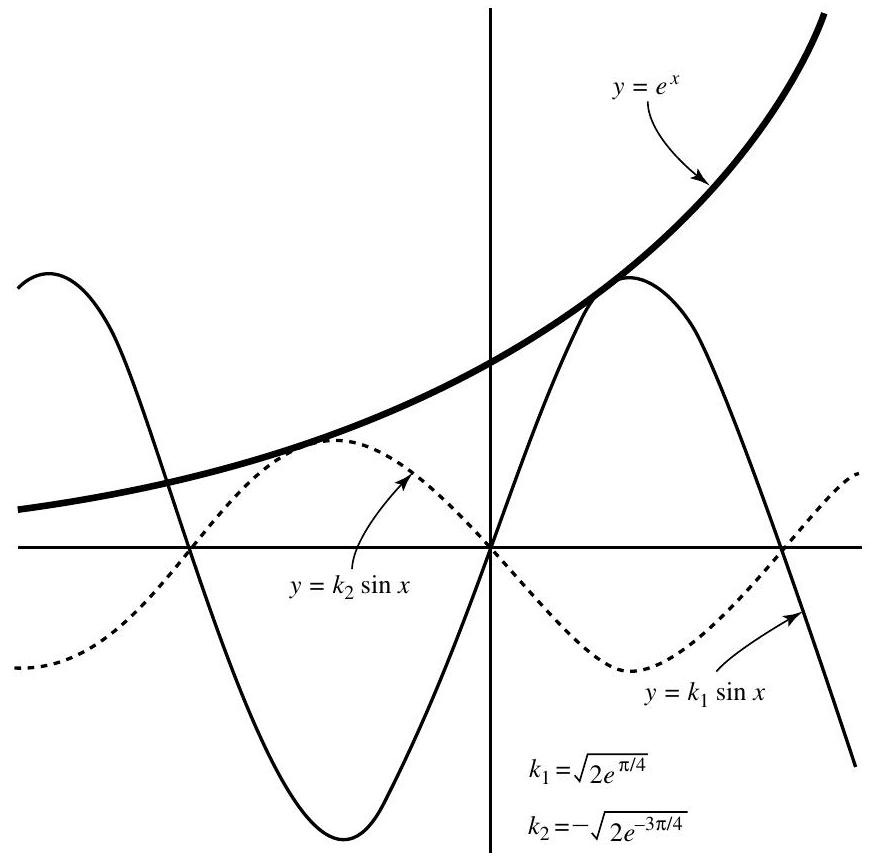
\includegraphics[width=0.70\linewidth]{calculus/images/4dd0024d-5e0f-40f8-af74-ec664288d8ef-23_864_873_299_644.jpg}
\end{center}
\end{solution}


\newpage





\question
The curve $2 x^{2} y+y^{2}=2 x+13$ passes through $(3,1)$ .Use the line tangent to the curve there to find the approximate value of $y$ at $x=2.8$ .
\begin{choices}
  \choice $0.5$
  \choice $0.9$
  \choice $0.95$
  \CorrectChoice $1.1$
  \choice $1.4$
\end{choices}
\begin{solution}
(D) We differentiate implicitly to find the slope $\dfrac{d y}{d x}$ :\\
$2\left(x^{2} \dfrac{d y}{d x}+2 x y\right)+2 y \dfrac{d y}{d x}=2$,\\
$\dfrac{d y}{d x}=\dfrac{1-2 x y}{x^{2}+y}$.\\
At $(3,1), \dfrac{d y}{d x}=-\dfrac{1}{2}$. The linearization is $y \simeq-\dfrac{1}{2}(x-3)+1$.
\end{solution}

\question
$\int \cos ^{3} x d x=$
\begin{choices}
  \choice $\dfrac{\cos ^{4} x}{4}+C$
  \choice $\dfrac{\sin ^{4} x}{4}+C$
  \CorrectChoice $\sin x-\dfrac{\sin ^{3} x}{3}+C$
  \choice $\sin x+\dfrac{\sin ^{3} x}{3}+C$
  \choice $\cos x-\dfrac{\cos ^{3} x}{3}+C$
\end{choices}
\begin{solution}
(C) $\int \cos ^{3} x d x=\int \cos ^{2} x \cdot \cos x d x=\int\left(1-\sin ^{2} x\right) \cos x d x$
\[
=\int \cos x d x-\int \sin ^{2} x \cdot \cos x d x=\sin x-\dfrac{\sin ^{3} x}{3}+C
\]
\end{solution}


\newpage





\question
The region bounded by $y=\tan x, y=0$ ,and $x=\dfrac{\pi}{4}$ is rotated about the $x$-axis.The volume generated equals
\begin{choices}
  \CorrectChoice $\pi-\dfrac{\pi^{2}}{4}$
  \choice $\pi(\sqrt{2}-1)$
  \choice $\dfrac{3 \pi}{4}$
  \choice $\pi\left(1+\dfrac{\pi}{4}\right)$
  \choice none of these
\end{choices}
\begin{solution}
About the $x$-axis. Disk.


\[
\begin{aligned}
\Delta V &= \pi y^{2} \Delta x \\
V &= \pi \displaystyle\int_{0}^{\pi / 4} \tan ^{2} x\, d x
   = \pi \displaystyle\int_{0}^{\pi / 4}\left(\sec ^{2} x-1\right) d x
   = \pi[\tan x-x]_{0}^{\pi / 4}
   = \pi\left(1-\dfrac{\pi}{4}\right)
\end{aligned}
\]


\end{solution}

\question
$\lim\limits_{h \to 0} \dfrac{a^{h}-1}{h}$ ,for the constant $a>0$ ,equals
\begin{choices}
  \choice $1$
  \choice $a$
  \CorrectChoice $\ln a$
  \choice $\log_{10} a$
  \choice $a \ln a$
\end{choices}
\begin{solution}
Let $f(x)=a^{x}$; then $\lim\limits_{h \to 0} \dfrac{a^{h}-1}{h}=\lim\limits_{h \to 0} \dfrac{a^{0+h}-a^{0}}{h}=f^{\prime}(0)=a^{0} \ln a=\ln a$.
\end{solution}


\newpage





\question
Solutions of the differential equation whose slope field is shown here are most likely to be
\begin{center}
  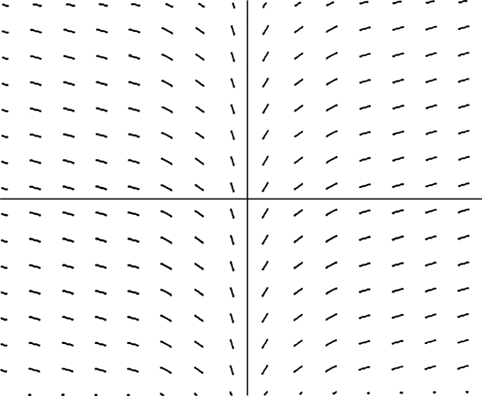
\includegraphics[width=0.40\linewidth]{calculus/images/more03.png}
\end{center}
\begin{choices}
  \choice quadratic
  \choice cubic
  \choice sinusoidal
  \choice exponential
  \CorrectChoice logarithmic
\end{choices}
\begin{solution}
$\dfrac{d y}{d x}$ is a function of $x$ alone; curves appear to be asymptotic to the $y$-axis and to increase more slowly as $|x|$ increases.
\end{solution}

\question
$\lim\limits_{h \to 0} \dfrac{1}{h} \displaystyle\int_{\dfrac{\pi}{4}}^{\dfrac{\pi}{4}+h} \dfrac{\sin x}{x} d x=$
\begin{choices}
  \choice $0$
  \choice $1$
  \choice $\dfrac{\sqrt{2}}{2}$
  \CorrectChoice $\dfrac{2 \sqrt{2}}{\pi}$
  \choice $\dfrac{2 \sqrt{2}(\pi-4)}{\pi^{2}}$
\end{choices}
\begin{solution}
The given limit is equivalent to
\[
\lim\limits_{h \to 0} \dfrac{\left(\dfrac{\pi}{4}+h\right)-F\left(\dfrac{\pi}{4}\right)}{h}=F^{\prime}\left(\dfrac{\pi}{4}\right),
\]
where $F^{\prime}(x)=\dfrac{\sin x}{x}$. The answer is $\dfrac{2 \sqrt{2}}{\pi}$.
\end{solution}


\newpage





\question
The graph of $g$, shown below, consists of the arcs of two quarter-circles and two straight-line segments. The value of $\displaystyle\int_{0}^{12} g(x) d x$ is\\
\begin{center}
  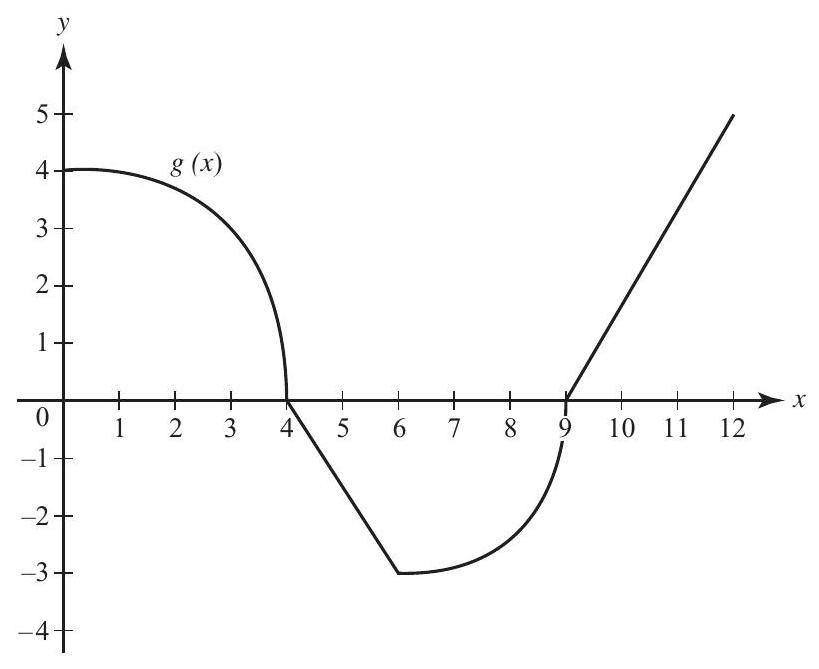
\includegraphics[width=0.40\linewidth]{calculus/images/4dd0024d-5e0f-40f8-af74-ec664288d8ef-06_669_819_454_937.jpg}
\end{center}
\begin{choices}
  \choice $\pi+2$
  \CorrectChoice $\dfrac{7 \pi}{4}+\dfrac{9}{2}$
  \choice $\dfrac{7 \pi}{4}+8$
  \choice $7 \pi+\dfrac{9}{2}$
  \choice $\dfrac{25 \pi}{4}+\dfrac{21}{2}$
\end{choices}
\begin{solution}
(B) $\displaystyle\int_{0}^{12} g(x) d x=\displaystyle\int_{0}^{4} g(x) d x+\displaystyle\int_{4}^{6} g(x) d x+\displaystyle\int_{6}^{9} g(x) d x+\displaystyle\int_{9}^{12} g(x) d x$
\[
=4 \pi-3-\dfrac{9 \pi}{4}+\dfrac{15}{2} .
\]
\end{solution}


\newpage





\question
Which of these could be a particular solution of the differential equation whose slope field is shown here?
\begin{center}
  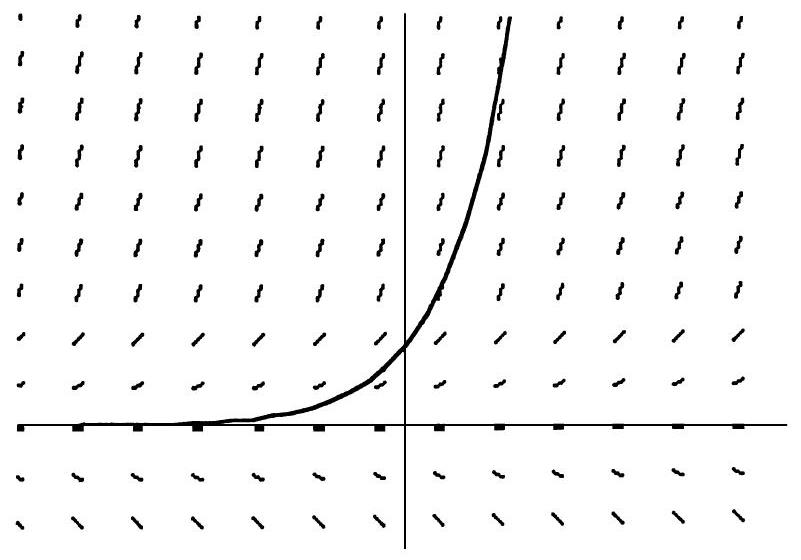
\includegraphics[width=0.40\linewidth]{calculus/images/4dd0024d-5e0f-40f8-af74-ec664288d8ef-24_560_801_988_960.jpg}
\end{center}
\begin{choices}
  \choice $y=\dfrac{1}{x}$
  \choice $y=\ln x$
  \CorrectChoice $y=e^{x}$
  \choice $y=e^{-x}$
  \choice $y=e^{x^{2}}$
\end{choices}
\begin{solution}
In the figure, the curve for $y=e^{x}$ has been superimposed on the slope field.\\
\begin{center}
  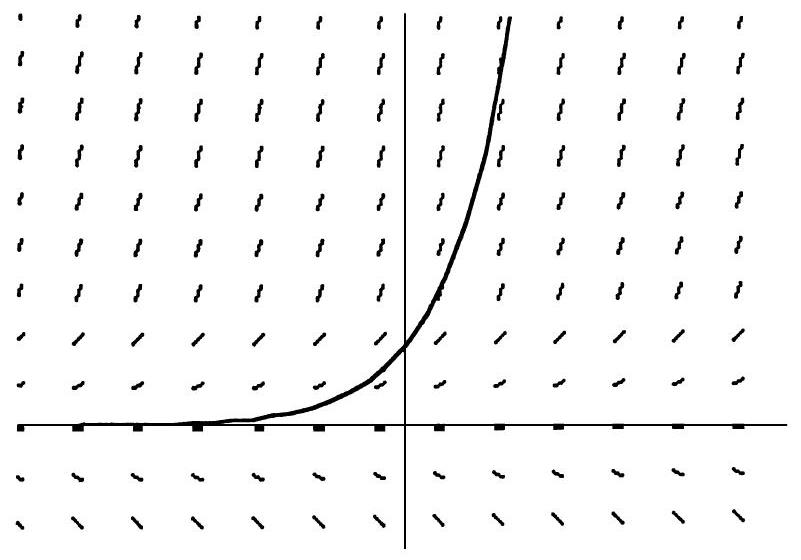
\includegraphics[width=0.40\linewidth]{calculus/images/4dd0024d-5e0f-40f8-af74-ec664288d8ef-24_560_801_988_960.jpg}
\end{center}
\end{solution}

\question
What is the domain of the particular solution for $\dfrac{d y}{d x}=\dfrac{6 x}{x^{2}-4}$ containing the point where $x=-1$ ?
\begin{choices}
  \choice $x<0$
  \choice $x>-2$
  \CorrectChoice $-2<x<2$
  \choice $x \neq \pm 2$
  \choice none of these; no solution exists for $x=-1$
\end{choices}
\begin{solution}
The general solution is $y=3 \ln \left|x^{2}-4\right|+C$. The differential equation $\dfrac{d y}{d x}=\dfrac{6 x}{x^{2}-4}$ reveals that the derivative does not exist for $x= \pm 2$. The particular solution must be differentiable in an interval containing initial value $x=-1$, so the domain is $-2<x<2$.
\end{solution}




\newpage






\question
The slope field shown here is for the differential equation\\
\begin{center}
  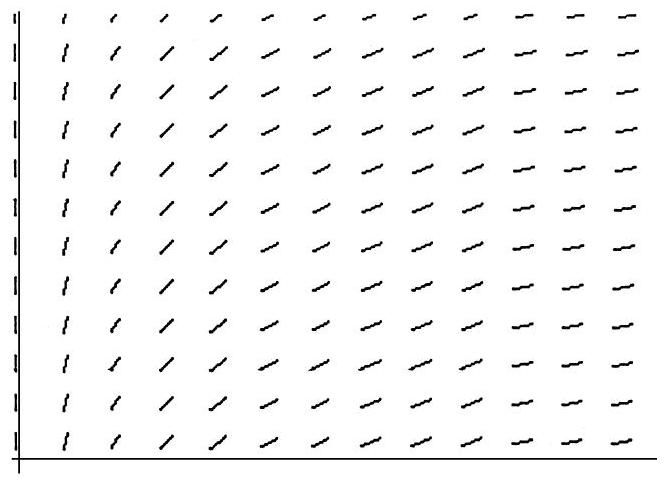
\includegraphics[width=0.40\linewidth]{calculus/images/4dd0024d-5e0f-40f8-af74-ec664288d8ef-07_483_667_378_663.jpg}
\end{center}
\begin{choices}
  \CorrectChoice $y^{\prime}=\dfrac{1}{x}$
  \choice $y^{\prime}=\ln x$
  \choice $y^{\prime}=e^{x}$
  \choice $y^{\prime}=y$
  \choice $y^{\prime}=-y^{2}$
\end{choices}
\begin{solution}
The solution curve shown is $y=\ln x$, so the differential equation is $y^{\prime}=\dfrac{1}{x}$.
\begin{center}
  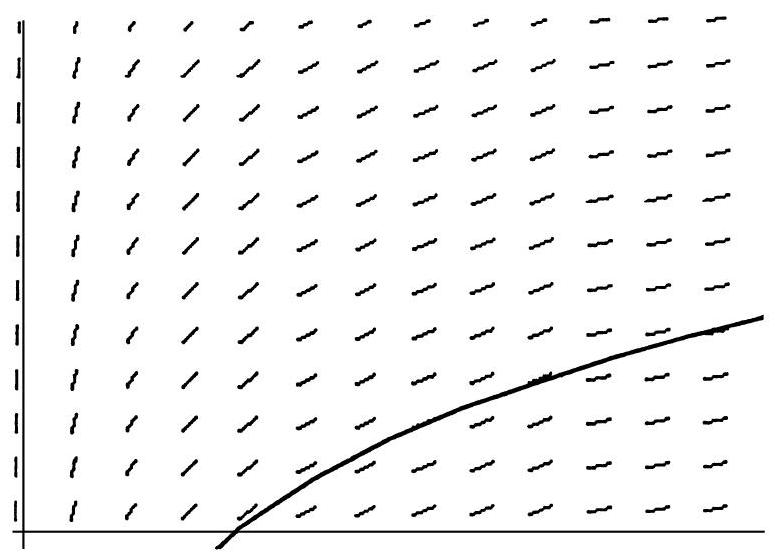
\includegraphics[width=0.40\linewidth]{calculus/images/4dd0024d-5e0f-40f8-af74-ec664288d8ef-24_560_780_1953_967.jpg}
\end{center}
\end{solution}


\newpage





\question
If we substitute $x=\tan \theta$, which of the following is equivalent to $\displaystyle\int_{0}^{1} \sqrt{1+x^{2}} d x$ ?
\begin{choices}
  \choice $\displaystyle\int_{0}^{1} \sec \theta d \theta$
  \choice $\displaystyle\int_{0}^{1} \sec ^{3} \theta d \theta$
  \choice $\displaystyle\int_{0}^{\pi / 4} \sec \theta d \theta$
  \CorrectChoice $\displaystyle\int_{0}^{\pi / 4} \sec ^{3} \theta d \theta$
  \choice $\displaystyle\int_{0}^{\tan 1} \sec ^{3} \theta d \theta$
\end{choices}
\begin{solution}
(D) $\sqrt{1+\tan ^{2} \theta}=\sec \theta ; d x=\sec ^{2} \theta ; 0 \leqslant x \leqslant 1$; so $0 \leq \theta \leq \dfrac{\pi}{4}$.
\end{solution}

\question
If $x=2 \sin u$ and $y=\cos 2 u$, then a single equation in $x$ and $y$ is
\begin{choices}
  \choice $x^{2}+y^{2}=1$
  \choice $x^{2}+4 y^{2}=4$
  \CorrectChoice $x^{2}+2 y=2$
  \choice $x^{2}+y^{2}=4$
  \choice $x^{2}-2 y=2$
\end{choices}
\begin{solution}
(C) The equations may be rewritten as $\dfrac{x}{2}=\sin u$ and $y=1-2 \sin ^{2} u$, giving $y=1-2 \cdot \dfrac{x^{2}}{2}$.
\end{solution}

\question
The area bounded by the lemniscate with polar equation $r^{2}=2 \cos 2 \theta$ is equal to
\begin{choices}
  \choice $4$
  \choice $1$
  \choice $\dfrac{1}{4}$
  \CorrectChoice $2$
  \choice none of these
\end{choices}
\begin{solution}
(D) Use the formula for area in polar coordinates,
\[
A=\dfrac{1}{2} \displaystyle\int_{\alpha}^{\beta} r^{2} d \theta
\]
then the required area is given by
\[
4 \cdot \dfrac{1}{2} \displaystyle\int_{0}^{\pi / 4} 2 \cos 2 \theta
\]
(See polar graph 63 in the Appendix.)
\end{solution}


\newpage





\question
$\displaystyle\int_{-\infty}^{\infty} \dfrac{d x}{x^{2}+1}=$
\begin{choices}
  \choice $0$
  \choice $\dfrac{\pi}{2}$
  \CorrectChoice $\pi$
  \choice $2 \pi$
  \choice none of these
\end{choices}
\begin{solution}
(C) $\quad \displaystyle\int_{-\infty}^{\infty} \dfrac{d x}{x^{2}+1}=\left.\lim\limits_{b \to \infty} \tan ^{-1} x\right|_{-b} ^{b}=\dfrac{\pi}{2}-\left(-\dfrac{\pi}{2}\right)=\pi$.
\end{solution}

\question
The first four terms of the Maclaurin series (the Taylor series about $x=0$ ) for $f(x)=\dfrac{1}{1-2 x}$ are
\begin{choices}
  \CorrectChoice $1+2 x+4 x^{2}+8 x^{3}$
  \choice $1-2 x+4 x^{2}-8 x^{3}$
  \choice $-1-2 x-4 x^{2}-8 x^{3}$
  \choice $1-x+x^{2}-x^{3}$
  \choice $1+x+x^{2}+x^{3}$
\end{choices}
\begin{solution}
(A) The first three derivatives of $\dfrac{1}{1-2 x}$ are $\dfrac{2}{(1-2 x)^{2}}, \dfrac{8}{(1-2 x)^{3}}$, and $\dfrac{48}{(1-2 x)^{4}}$.

The first four terms of the Maclaurin series (about $x=0$ ) are $1,+2 x$,\\
$+\dfrac{8 x^{2}}{2!}$, and $+\dfrac{48 x^{3}}{3!}$.\\
Note also that $\dfrac{1}{1-2 x}$ represents the sum of an infinite geometric series with first term 1 and common ratio $2 x$. Hence,
\[
\dfrac{1}{1-2 x}=1+2 x+(2 x)^{2}+(2 x)^{3}+\cdots
\]
\end{solution}


\newpage





\question
$\int x^{2} e^{-x} d x=$
\begin{choices}
  \choice $\dfrac{1}{3} x^{3} e^{-x}+C$
  \choice $-\dfrac{1}{3} x^{3} e^{-x}+C$
  \choice $-x^{2} e^{-x}+2 x e^{-x}+C$
  \CorrectChoice $-x^{2} e^{-x}-2 x e^{-x}-2 e^{-x}+C$
  \choice $-x^{2} e^{-x}+2 x e^{-x}-2 e^{-x}+C$


\end{choices}
\begin{solution}
We use parts, first letting $u=x^{2}, d v=e^{-x} d x$; then $d u=2 x d x, v=-e^{-x}$ and
\[
\int x^{2} e^{-x} d x=-x^{2} e^{-x}+2 \int x e^{-x} d x
\]
Now we use parts again, letting $u=x, d v=e^{-x} d x$; then $d u=d x, v=-e^{-x}$ and
\[
-x^{2} e^{-x}+2 \int x e^{-x} d x=-x^{2} e^{-x}+2\left(-x e^{-x}+\int e^{-x} d x\right)
\]
Then $\int x^{2} e^{-x} d x=x^{2}\left(-e^{-x}\right)-(2 x) e^{-x}+2\left(-e^{-x}\right)+C$
\end{solution}

\question
$\displaystyle\int_{0}^{\pi / 2} \sin ^{2} x d x$ is equal to
\begin{choices}
  \choice $\dfrac{1}{3}$
  \choice $\dfrac{\pi}{4}-\dfrac{1}{4}$
  \choice $\dfrac{\pi}{2}$
  \choice $\dfrac{\pi}{2}-\dfrac{1}{3}$
  \CorrectChoice $\dfrac{\pi}{4}$
\end{choices}
\begin{solution}
(E) Use formula (20) in the Appendix to rewrite the integral as
\[
\dfrac{1}{2} \displaystyle\int_{0}^{\pi / 2}(1-\cos 2 x) d x=\left.\dfrac{1}{2}\left(x-\dfrac{\sin 2 x}{2}\right)\right|_{0} ^{\pi / 2}=\dfrac{1}{2}\left(\dfrac{\pi}{2}\right)
\]
\end{solution}





\newpage





\question
A curve is given parametrically by the equations $x=t, y=1-\cos t$. The area bounded by the curve and the $x$-axis on the interval $0 \leqq t \leqq 2 \pi$ is equal to
\begin{choices}
  \choice $2(\pi+1)$
  \choice $\pi$
  \choice $4 \pi$
  \choice $\pi+1$
  \CorrectChoice $2 \pi$
\end{choices}
\begin{solution}
The area, $A$, is represented by $\displaystyle\int_{0}^{2 \pi}(1-\cos t)=2 \pi$.
\end{solution}

\question
If $x=a \cot \theta$ and $y=a \sin ^{2} \theta$, then $\dfrac{d y}{d x}$, when $\theta=\dfrac{\pi}{4}$, is equal to
\begin{choices}
  \choice $\dfrac{1}{2}$
  \choice $-1$
  \choice $2$
  \CorrectChoice $-\dfrac{1}{2}$
  \choice $-\dfrac{1}{4}$
\end{choices}
\begin{solution}
$\dfrac{d y}{d x}=\dfrac{\dfrac{d y}{d \theta}}{\dfrac{d x}{d \theta}}=\dfrac{2 a \sin \theta \cos \theta}{-a \csc ^{2} \theta}=-2 \sin ^{3} \theta \cos \theta$.
\end{solution}

\question
Which of the following improper integrals diverges?
\begin{choices}
  \choice $\displaystyle\int_{0}^{\infty} e^{-x^{2}} d x$
  \choice $\displaystyle\int_{-\infty}^{0} e^{x} d x$
  \CorrectChoice $\displaystyle\int_{0}^{1} \dfrac{d x}{x}$
  \choice $\displaystyle\int_{0}^{\infty} e^{-x} d x$
  \choice $\displaystyle\int_{0}^{1} \dfrac{d x}{\sqrt{x}}$
\end{choices}
\begin{solution}
Check to verify that each of the other improper integrals converges.
\end{solution}





\newpage





\question
$\displaystyle\int_{2}^{4} \dfrac{d u}{\sqrt{16-u^{2}}}$ equals
\begin{choices}
  \choice $\dfrac{\pi}{12}$
  \choice $\dfrac{\pi}{6}$
  \choice $\dfrac{\pi}{4}$
  \CorrectChoice $\dfrac{\pi}{3}$
  \choice $\dfrac{2 \pi}{3}$
\end{choices}
\begin{solution}
Note that the integral is improper.


\[
\lim\limits_{k \to 4^{-}} \displaystyle\int_{2}^{k} \dfrac{d u}{\sqrt{16-u^{2}}}=\lim\limits_{k \to 4^{-}} \dfrac{1}{4} \displaystyle\int_{2}^{k} \dfrac{d u}{\sqrt{1-\dfrac{u^{2}}{16}}}=\lim\limits_{k \to 4^{-}} \dfrac{1}{4} \cdot 4 \displaystyle\int_{2}^{k} \dfrac{\dfrac{1}{4} d u}{\sqrt{1-\dfrac{u^{2}}{16}}}=\left.\lim\limits_{k \to 4^{-}} \sin \dfrac{u}{4}\right|_{2} ^{k}=\dfrac{\pi}{3}
\]

See Example 26, page 312.
\end{solution}

\question
$\lim\limits_{x \to 0^{+}}\left(\dfrac{1}{x}\right)^{x}$ is
\begin{choices}
  \choice $-\infty$
  \choice $0$
  \CorrectChoice $1$
  \choice $\infty$
  \choice nonexistent
\end{choices}
\begin{solution}
(C) Let $y=\left(\dfrac{1}{x}\right)^{x}$. Then $\ln y=-x \ln x$ and

\[
\lim\limits_{x \to 0^{+}} \ln y=\lim\limits_{x \to 0^{+}} \dfrac{-\ln x}{1 / x}
\]

Now apply L'Hpital's Rule:

\[
\lim\limits_{x \to 0^{+}} \ln y=\lim\limits_{x \to 0^{+}} \dfrac{-1 / x}{-1 / x^{2}}=0
\]

So, if $\lim\limits_{x \to 0^{+}} \ln y=0$, then $\lim\limits_{x \to 0^{+}} y=1$.
\end{solution}





\newpage





\question
A particle moves along the parabola $x=3 y-y^{2}$ so that $\dfrac{d y}{d t}=3$ at all time $t$. The speed of the particle when it is at position $(2,1)$ is equal to
\begin{choices}
  \choice $0$
  \choice $3$
  \choice $\sqrt{13}$
  \CorrectChoice $3 \sqrt{2}$
  \choice none of these
\end{choices}
\begin{solution}
(D) The speed, $|\mathbf{v}|$, equals $\sqrt{\left(\dfrac{d x}{d t}\right)^{2}+\left(\dfrac{d y}{d t}\right)^{2}}$, and since $x=3 y-y^{2}$,

\[
\dfrac{d x}{d t}=(3-2 y) \dfrac{d x}{d t}=(3-2 y) \cdot 3
\]

Then $|\mathbf{v}|$ is evaluated, using $y=1$, and equals $\sqrt{(3)^{2}+(3)^{2}}$.
\end{solution}

\question
$\lim\limits_{x \to 0^{+}} \dfrac{\cot x}{\ln x}=$
\begin{choices}
  \CorrectChoice $-\infty$
  \choice $-1$
  \choice $0$
  \choice $1$
  \choice $\infty$
\end{choices}
\begin{solution}
(A) This is an indeterminate form of type $\dfrac{\infty}{\infty}$; use L'Hpital's Rule:
\[
\lim\limits_{x \to 0^{+}} \dfrac{\cot x}{\ln x}=\lim\limits_{x \to 0^{+}} \dfrac{-\csc ^{2} x}{1 / x}=\lim\limits_{x \to 0^{+}} \dfrac{x}{\sin x} \cdot \dfrac{-1}{\sin x}=-\infty
\]
\end{solution}


\newpage





\question
When rewritten as partial fractions, $\dfrac{3 x+2}{x^{2}-x-12}$ includes which of the following?

\statementbox{%
\begin{enumerate}
\renewcommand{\labelenumi}{\Roman{enumi}.}
\item $\dfrac{1}{x+3}$
\item $\dfrac{1}{x-4}$
\item $\dfrac{2}{x-4}$
\end{enumerate}%
}
\begin{choices}
  \choice none
  \choice I only
  \choice II only
  \choice III only
  \CorrectChoice I and III
\end{choices}
\begin{solution}
We find $A$ and $B$ such that $\dfrac{3 x+2}{(x+3)(x-4)}=\dfrac{A}{x+3}+\dfrac{B}{x-4}$.


After multiplying by the common denominator, we have

\[
3 x+2=A(x-4)+B(x+3)
\]

Substituting $x=-3$ yields $A=1$, and $x=4$ yields $B=2$; hence,

\[
\dfrac{3 x+2}{x^{2}-x-12}=\dfrac{1}{x+3}+\dfrac{2}{x-4} .
\]


\end{solution}

\question
Using two terms of an appropriate Maclaurin series, estimate $\displaystyle\int_{0}^{1} \dfrac{1-\cos x}{x} d x$.
\begin{choices}
  \choice $\dfrac{1}{96}$
  \CorrectChoice $\dfrac{23}{96}$
  \choice $\dfrac{1}{4}$
  \choice $\dfrac{25}{96}$
  \choice undefined; the integral is improper
\end{choices}
\begin{solution}
Since $\cos x \simeq 1-\dfrac{x^{2}}{2!}+\dfrac{x^{4}}{4!}, \dfrac{1-\cos x}{x} \simeq \dfrac{x}{2}-\dfrac{x^{3}}{4!}$.\\
Then $\left.\displaystyle\int_{0}^{1} \dfrac{1-\cos x}{x} d x \simeq\left(\dfrac{x^{2}}{4}-\dfrac{x^{4}}{96}\right)\right|_{0} ^{1}=\dfrac{1}{4}-\dfrac{1}{96}$.\\
Note that $\lim\limits_{x \to 0^{+}} \dfrac{1-\cos x}{x}=0$, so the integral is proper.
\end{solution}





\newpage





\question
The slope of the spiral $r=\theta$ at $\theta=\dfrac{\pi}{4}$ is
\begin{choices}
  \choice $-\sqrt{2}$
  \choice $-1$
  \choice $1$
  \CorrectChoice $\dfrac{4+\pi}{4-\pi}$
  \choice undefined
\end{choices}
\begin{solution}
(D) We represent the spiral as $P(\theta)=(\theta \cos \theta, \theta \sin \theta)$. So
\[
\dfrac{d y}{d x}=\dfrac{d y / d \theta}{d x / d \theta}=\dfrac{\theta \cos \theta+\sin \theta}{-\theta \sin \theta+\cos \theta}=\dfrac{\dfrac{\pi}{4} \cdot \dfrac{\sqrt{2}}{2}+\dfrac{\sqrt{2}}{2}}{-\dfrac{\pi}{4} \cdot \dfrac{\sqrt{2}}{2}+\dfrac{\sqrt{2}}{2}}=\dfrac{\pi / 4+1}{-\pi / 4+1}
\]
\end{solution}





\newpage





\question
The graph of function $h$ is shown here. Which of these statements is (are) true?
\begin{center}
  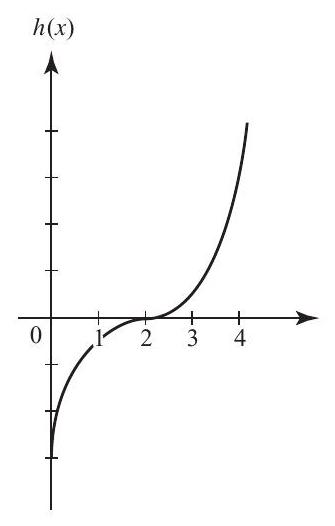
\includegraphics[width=0.40\linewidth]{calculus/images/4dd0024d-5e0f-40f8-af74-ec664288d8ef-09_526_335_971_1347.jpg}
\end{center}

\statementbox{%
\begin{enumerate}
\renewcommand{\labelenumi}{\Roman{enumi}.}
\item The first derivative is never negative.
\item The second derivative is constant.
\item The first and second derivatives equal 0 at the same point.
\end{enumerate}%
}
\begin{choices}
  \choice I only
  \choice III only
  \choice I and II
  \CorrectChoice I and III
  \choice all three
\end{choices}
\begin{solution}
Since $h$ is increasing, $h^{\prime} \geq 0$. The graph of $h$ is concave downward for $x<2$ and upward for $x>2$, so $h^{\prime \prime}$ changes sign at $x=2$, where it appears that $h^{\prime}=0$ also.
\end{solution}



\newpage



\question
Graphs of functions $f(x), g(x)$, and $h(x)$ are shown below.\\
\begin{center}
  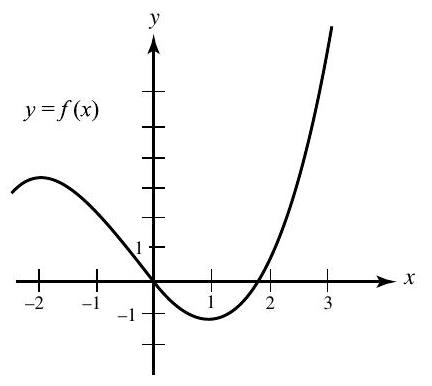
\includegraphics[width=0.30\linewidth]{calculus/images/4dd0024d-5e0f-40f8-af74-ec664288d8ef-09_386_432_1639_315.jpg}
  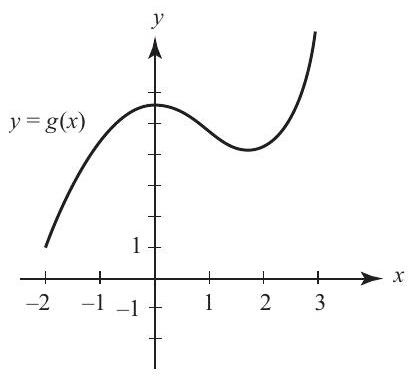
\includegraphics[width=0.30\linewidth]{calculus/images/4dd0024d-5e0f-40f8-af74-ec664288d8ef-09_383_418_1642_784.jpg}
  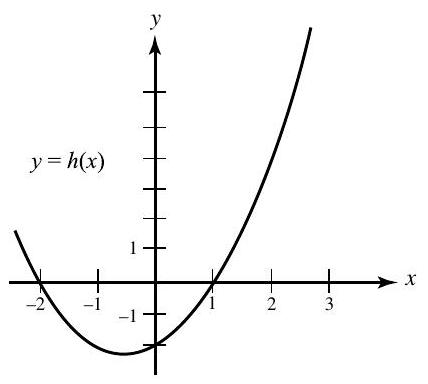
\includegraphics[width=0.30\linewidth]{calculus/images/4dd0024d-5e0f-40f8-af74-ec664288d8ef-09_384_428_1637_1247.jpg}
\end{center}

Consider the following statements:

\statementbox{%
\begin{enumerate}
\renewcommand{\labelenumi}{\Roman{enumi}.}
\item $g(x)=f^{\prime}(x)$
\item $f(x)=g^{\prime}(x)$
\item $h(x)=g^{\prime \prime}(x)$
\end{enumerate}%
}

Which of these statements is (are) true?
\begin{choices}
  \choice I only
  \choice II only
  \CorrectChoice II and III only
  \choice all three
  \choice none of these
\end{choices}
\begin{solution}
I is false since, for example, $f^{\prime}(-2)=f^{\prime}(1)=0$ but neither $g(-2)$ nor $g(1)$ equals zero.\\
II is true. Note that $f=0$ where $g$ has relative extrema, and $f$ is positive, negative, then positive on intervals where $g$ increases, decreases, then increases.\\
III is also true. Check the concavity of $g$ : when the curve is concave down, $h<0$; when up, $h>0$.
\end{solution}


\newpage





\question
If $y=\displaystyle\int_{3}^{x} \dfrac{1}{\sqrt{3+2 t}} d t$, then $\dfrac{d^{2} y}{d x^{2}}=$
\begin{choices}
  \CorrectChoice $-\dfrac{1}{(3+2 x)^{\dfrac{3}{2}}}$
  \choice $\dfrac{3}{(3+2 x)^{\dfrac{5}{2}}}$
  \choice $\dfrac{\sqrt{3+2 x}}{2}$
  \choice $\dfrac{(3+2 x)^{\dfrac{3}{2}}}{3}$
  \choice $0$
\end{choices}
\begin{solution}
(A) If $y=\displaystyle\int_{3}^{x} \dfrac{1}{\sqrt{3+2 t}} d t$, then $\dfrac{d y}{d x}=\dfrac{1}{\sqrt{3+2 x}}$, so $\dfrac{d^{2} y}{d x^{2}}=-\dfrac{1}{2}(3+2 x)^{-3 / 2}(2)$.
\end{solution}

\question
If $\displaystyle\int_{-3}^{4} f(x) d x=6$, then $\displaystyle\int_{-4}^{3} f(x+1) d x=$
\begin{choices}
  \choice $-6$
  \choice $-5$
  \choice $5$
  \CorrectChoice $6$
  \choice $7$
\end{choices}
\begin{solution}
(D) $\displaystyle\int_{-4}^{3} f(x+1) d x$ represents the area of the same region as $\displaystyle\int_{-3}^{4} f(x) d x$, translated one unit to the left.
\end{solution}

\question
At what point in the interval $[1,1.5]$ is the rate of change of $f(x)=\sin x$ equal to its average rate of change on the interval?
\begin{choices}
  \choice $0.995$
  \choice $1.058$
  \choice $1.239$
  \CorrectChoice $1.253$
  \choice $1.399$
\end{choices}
\begin{solution}
(D) According to the Mean Value Theorem, there exists a number $c$ in the interval $[1,1.5]$ such that $f^{\prime}(c)=\dfrac{f(1.5)-f(1)}{1.5-1}$. Use your calculator to solve the equation $\cos c=\dfrac{\sin 1.5-\sin 1}{0.5}$ for $c$ (in radians).
\end{solution}



\newpage






\question\label{calc11:f-sign-lines}
Suppose $f^{\prime}(x)=x^{2}(x-1)$. Then $f^{\prime \prime}(x)=x(3 x-2)$. Over which interval(s) is the graph of $f$ both increasing and concave up?

\statementbox{%
\begin{enumerate}
\renewcommand{\labelenumi}{\Roman{enumi}.}
\item $x<0$
\item $0<x<\dfrac{2}{3}$
\item $\dfrac{2}{3}<x<1$
\item $x>1$
\end{enumerate}%
}
\begin{choices}
  \choice I only
  \choice II only
  \choice II and IV
  \choice I and III
  \CorrectChoice IV only
\end{choices}
\begin{solution}
(E) Here are the relevant sign lines:\\
\begin{center}
  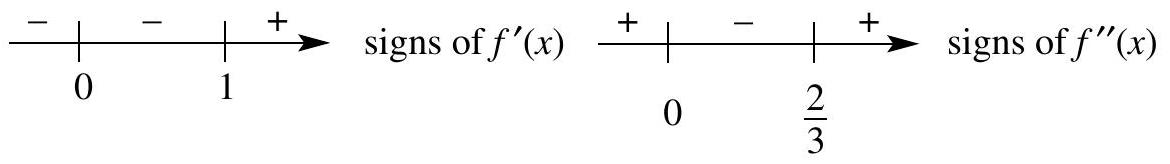
\includegraphics[width=0.70\linewidth]{calculus/images/4dd0024d-5e0f-40f8-af74-ec664288d8ef-28_164_1170_688_862.jpg}
\end{center}

We see that $f^{\prime}$ and $f^{\prime \prime}$ are both positive only if $x>1$.
\end{solution}

\question\label{calc11:f-graph}
Which of the following statements is true about the graph of $f(x)$?
\begin{choices}
  \choice The graph has no relative extrema.
  \choice The graph has one relative extremum and one inflection point.
  \choice The graph has two relative extrema and one inflection point.
  \choice The graph has two relative extrema and two inflection points.
  \CorrectChoice None of the preceding statements is true.
\end{choices}
\begin{solution}
(E) Note from the sign lines in Question~\ref{calc11:f-sign-lines} that $f$ changes from decreasing to increasing at $x=1$, so $f$ has a local minimum.

Also, the graph of $f$ changes from concave up to concave down at $x=0$, then back to concave up at $x=\dfrac{2}{3}$; hence $f$ has two points of inflection.
\end{solution}


\newpage





\question
The $n$th derivative of $\ln (x+1)$ at $x=2$ equals
\begin{choices}
  \choice $\dfrac{(-1)^{n-1}}{3^{n}}$
  \choice $\dfrac{(-1)^{n} \cdot n!}{3^{n+1}}$
  \CorrectChoice $\dfrac{(-1)^{n-1}(n-1)!}{3^{n}}$
  \choice $\dfrac{(-1)^{n+1} \cdot n!}{3^{n+1}}$
  \choice $\dfrac{(-1)^{n+1}}{3^{n+1}}$
\end{choices}
\begin{solution}
(C) The derivatives of $\ln (x+1)$ are $\dfrac{1}{x+1}, \dfrac{-1}{(x+1)^{2}}, \dfrac{+2!}{(x+1)^{3}}, \dfrac{-(3!)}{(x+1)^{4}}, \ldots$ The $n$th derivative at $x=2$ is $\dfrac{(-1)^{n-1}(n-1)!}{3^{n}}$.
\end{solution}

\question
If $f(x)$ is continuous at the point where $x=a$, which of the following statements may be false?
\begin{choices}
  \choice $\lim\limits_{x \to a} f(x)$ exists.
  \choice $\lim\limits_{x \to a} f(x)=f(a)$.
  \CorrectChoice $f^{\prime}(a)$ exists.
  \choice $f(a)$ is defined.
  \choice $\lim\limits_{x \to a^{-}} f(x)=\lim\limits_{x \to a^{+}} f(x)$.
\end{choices}
\begin{solution}
(C) The absolute-value function $f(x)=|x|$ is continuous at $x=0$, but $f^{\prime}(0)$ does not exist.
\end{solution}

\question
Suppose $\displaystyle\int_{0}^{3} f(x+k) d x=4$, where $k$ is a constant. Then $\displaystyle\int_{k}^{3+k} f(x) d x$ equals
\begin{choices}
  \choice $3$
  \choice $4-k$
  \CorrectChoice $4$
  \choice $4+k$
  \choice none of these
\end{choices}
\begin{solution}
(C) Let $F^{\prime}(x)=f(x)$; then $F^{\prime}(x+k)=f(x+k)$;

\[
\begin{aligned}
& \displaystyle\int_{0}^{3} f(x+k) d x=F(3+k)-F(k) \\
& \displaystyle\int_{k}^{3+k} f(x) d x=F(3+k)-F(k)
\end{aligned}
\]

Or let $u=x+k$. Then $d x=d u$; when $x=0, u=k$; when $x=3, u=3+k$.
\end{solution}

\question
The volume, in cubic feet, of an "inner tube" with inner diameter 4 ft and outer diameter 8 ft is
\begin{choices}
  \choice $4 \pi^{2}$
  \choice $12 \pi^{2}$
  \choice $8 \pi^{2}$
  \choice $24 \pi^{2}$
  \CorrectChoice $6 \pi^{2}$
\end{choices}
\begin{solution}
(E) See the figure. The equation of the generating circle is $(x-3)^{2}+y^{2}=1$, which yields $x=3 \pm \sqrt{1-y^{2}}$.\\
\begin{center}
  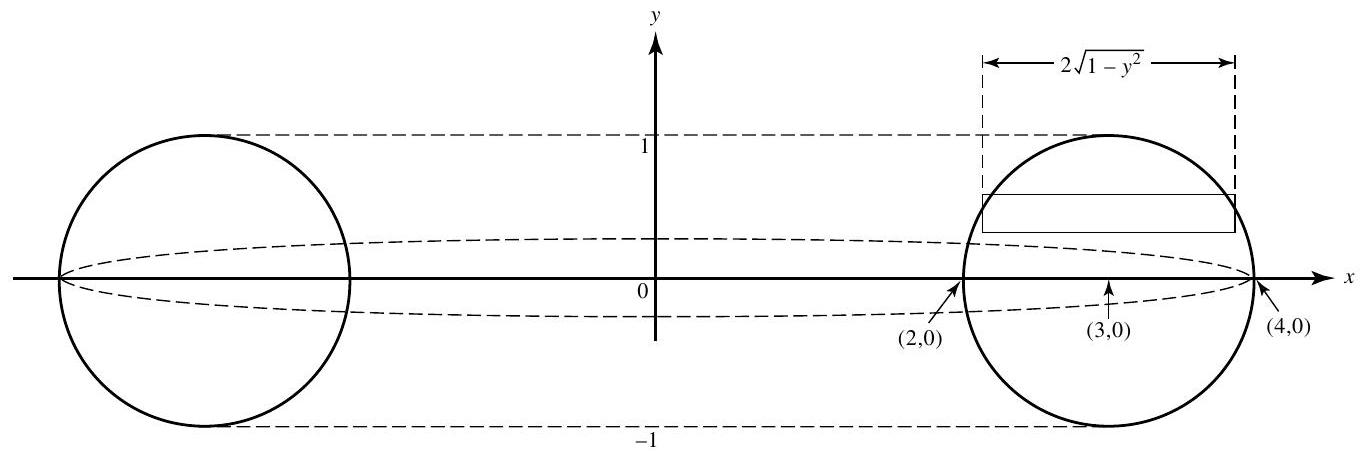
\includegraphics[width=0.70\linewidth]{calculus/images/4dd0024d-5e0f-40f8-af74-ec664288d8ef-28_458_1365_2173_672.jpg}
\end{center}
About the $y$-axis: $\Delta V=2 \pi \cdot 3 \cdot 2 \sqrt{1-y^{2}} \Delta y$.
\[
\text { Thus, } \begin{aligned}
V & =2 \displaystyle\int_{0}^{1} 12 \pi \sqrt{1-y^{2}} d y \\
& =24 \pi \text { times the area of a quarter of a unit circle }=6 \pi^{2}
\end{aligned}
\]
\end{solution}

\question
If $f(u)=\tan ^{-1} u^{2}$ and $g(u)=e^{u}$, then the derivative of $f(g(u))$ is
\begin{choices}
  \choice $\dfrac{2 u e^{u}}{1+u^{4}}$
  \choice $\dfrac{2 u e^{u^{2}}}{1+u^{4}}$
  \choice $\dfrac{2 e^{u}}{1+4 e^{2 u}}$
  \CorrectChoice $\dfrac{2 e^{2 u}}{1+e^{4 u}}$
  \choice $\dfrac{2 e^{2 u}}{\sqrt{1-e^{4 u}}}$
\end{choices}
\begin{solution}
Note that $f(g(u))=\tan ^{-1}\left(e^{2 u}\right)$; then the derivative is $\dfrac{1}{1+\left(e^{2 u}\right)^{2}}\left(2 e^{2 u}\right)$.
\end{solution}


\newpage



\question
If $\sin (x y)=y$, then $\dfrac{d y}{d x}$ equals
\begin{choices}
  \choice $\sec (x y)$
  \choice $y \cos (x y)-1$
  \choice $\dfrac{1-y \cos (x y)}{x \cos (x y)}$
  \CorrectChoice $\dfrac{y \cos (x y)}{1-x \cos (x y)}$
  \choice $\cos (x y)$
\end{choices}
\begin{solution}
Let $y^{\prime}=\dfrac{d y}{d x}$. Then $\cos (x y)\left[x y^{\prime}+y\right]=y^{\prime}$. Solve for $y^{\prime}$.
\end{solution}

\question
Let $x>0$. Suppose $\dfrac{d}{d x} f(x)=g(x)$ and $\dfrac{d}{d x} g(x)=f(\sqrt{x})$; then $\dfrac{d^{2}}{d x^{2}} f\left(x^{2}\right)=$
\begin{choices}
  \choice $f\left(x^{4}\right)$
  \choice $f\left(x^{2}\right)$
  \choice $2 x g\left(x^{2}\right)$
  \choice $\dfrac{1}{2 x} f(x)$
  \CorrectChoice $2 g\left(x^{2}\right)+4 x^{2} f(x)$
\end{choices}
\begin{solution}
$\dfrac{d^{2}}{d x^{2}} f\left(x^{2}\right)=\dfrac{d}{d x}\left[\dfrac{d}{d x} f\left(x^{2}\right)\right]=\dfrac{d}{d x}\left[\dfrac{d}{d x} f\left(x^{2}\right) \cdot \dfrac{d x^{2}}{d x}\right]=\dfrac{d}{d x}\left[g\left(x^{2}\right) \cdot 2 x\right]$
\[
\begin{aligned}
& =g\left(x^{2}\right) \dfrac{d}{d x}(2 x)+2 x \dfrac{d}{d x} g\left(x^{2}\right)=g\left(x^{2}\right) \cdot 2+2 x \dfrac{d}{d x^{2}} g\left(x^{2}\right) \dfrac{d x^{2}}{d x} \\
& =2 g\left(x^{2}\right)+2 x \cdot f\left(\sqrt{x^{2}}\right) \cdot 2 x=2 g\left(x^{2}\right)+4 x^{2} \cdot f(x)
\end{aligned}
\]
\begin{center}
  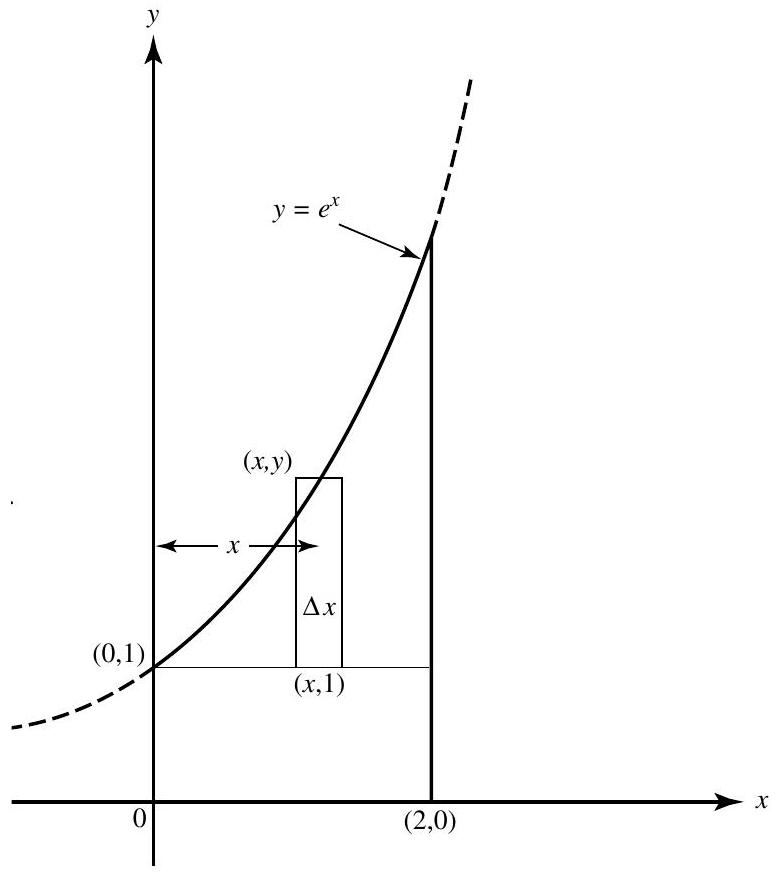
\includegraphics[width=0.40\linewidth]{calculus/images/4dd0024d-5e0f-40f8-af74-ec664288d8ef-29_875_778_1229_630.jpg}
\end{center}
\end{solution}



\newpage



\question
The region bounded by $y=e^{x}, y=1$, and $x=2$ is rotated about the $x$-axis. The volume of the solid generated is given by the integral
\begin{choices}
  \choice $\pi \displaystyle\int_{0}^{2} e^{2 x} d x$
  \choice $2 \pi \displaystyle\int_{1}^{e^{2}}(2-\ln y)(y-1) d y$
  \CorrectChoice $\pi \displaystyle\int_{0}^{2}\left(e^{2 x}-1\right) d x$
  \choice $2 \pi \displaystyle\int_{0}^{e^{2}} y(2-\ln y) d y$
  \choice $\pi \displaystyle\int_{0}^{2}\left(e^{x}-1\right)^{2} d x$
\end{choices}
\begin{solution}
(C) About the $x$-axis; see the figure. Washer.

\[
\begin{gathered}
\Delta V=\pi\left(y^{2}-1^{2}\right) \Delta x \\
V=\pi \displaystyle\int_{0}^{2}\left(e^{2 x}-1\right) d x
\end{gathered}
\]


\end{solution}

\question
Suppose the function $f$ is continuous on $1 \leqq x \leqq 2$, that $f^{\prime}(x)$ exists on $1<x<2$, that $f(1)=3$, and that $f(2)=0$. Which of the following statements is not necessarily true?
\begin{choices}
  \choice The Mean-Value Theorem applies to $f$ on $1 \leqq x \leqq 2$.
  \choice $\displaystyle\int_{1}^{2} f(x) d x$ exists.
  \CorrectChoice There exists a number $c$ in the closed interval $[1,2]$ such that $f^{\prime}(c)=0$.
  \choice If $k$ is any number between 0 and 3 , there is a number $c$ between 1 and 2 such that $f(c)=k$.
  \choice If $c$ is any number such that $1<c<2$, then $\lim\limits_{x \to c} f(x)$ exists.
\end{choices}
\begin{solution}
By the Mean Value Theorem, there is a number $c$ in $[1,2]$ such that
\[
f^{\prime}(c)=\dfrac{f(2)-f(1)}{2-1}=-3
\]
\end{solution}



\newpage



\question
The region $S$ in the figure is bounded by $y=\sec x$, the $y$-axis, and $y=4$. What is the volume of the solid formed when $S$ is rotated about the $y$-axis?\\
\begin{center}
  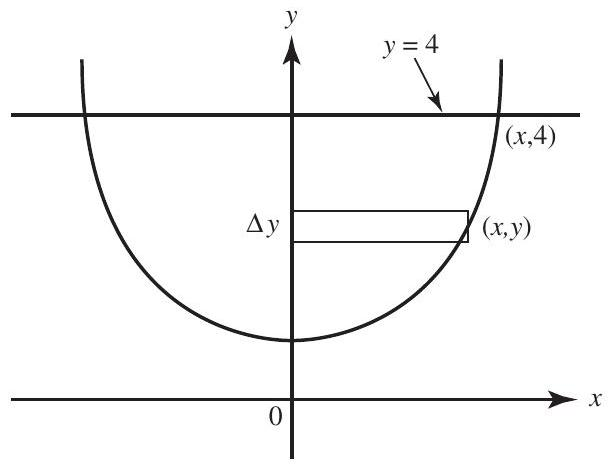
\includegraphics[width=0.40\linewidth]{calculus/images/4dd0024d-5e0f-40f8-af74-ec664288d8ef-12_467_611_433_1048.jpg}
\end{center}
\begin{choices}
  \choice $0.791$
  \choice $2.279$
  \choice $5.692$
  \CorrectChoice $11.385$
  \choice $17.217$
\end{choices}
\begin{solution}
The enclosed region, $S$, is bounded by $y=\sec x$, the $y$-axis, and $y=4$. It is to be rotated about the $y$-axis.\\
\begin{center}
  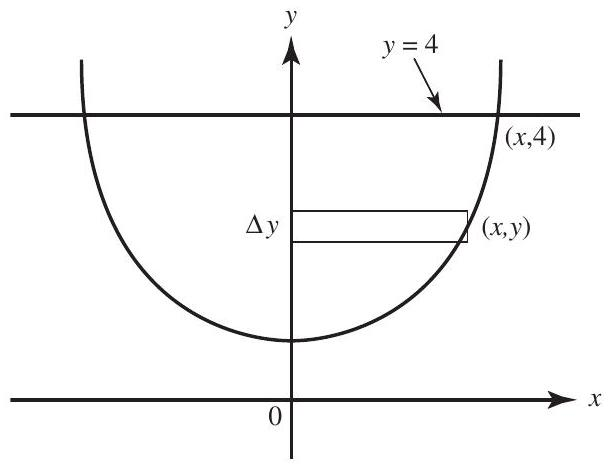
\includegraphics[width=0.40\linewidth]{calculus/images/4dd0024d-5e0f-40f8-af74-ec664288d8ef-30_470_615_417_1076.jpg}
\end{center}
Use disks; then $\Delta V=\pi R^{2} H=\pi(\operatorname{arc} \sec y)^{2} \Delta y$. Using the calculator, we find that
\[
\pi \displaystyle\int_{1}^{4}\left(\arccos \left(\dfrac{1}{y}\right)\right)^{2} d x \simeq 11.385
\]
\end{solution}





\newpage



\question
If 40 g of a radioactive substance decomposes to 20 g in 2 yr , then, to the nearest gram, the amount left after 3 yr is
\begin{choices}
  \choice $10$
  \choice $12$
  \CorrectChoice $14$
  \choice $16$
  \choice $17$
\end{choices}
\begin{solution}
If $Q$ is the amount at time $t$, then $Q=40 e^{-k t}$. Since $Q=20$ when $t=2$, $k=-0.3466$. Now find $Q$ when $t=3$, from $Q=40 e^{-(0.3466) 3}$, getting $Q=14$ to the nearest gram.
\end{solution}

\question
An object in motion along a line has acceleration $a(t)=\pi t+\dfrac{2}{1+t^{2}}$ and is at rest when $t=1$. Its average velocity from $t=0$ to $t=2$ is
\begin{choices}
  \CorrectChoice $0.362$
  \choice $0.274$
  \choice $3.504$
  \choice $7.008$
  \choice $8.497$
\end{choices}
\begin{solution}
The velocity $v(t)$ is an antiderivative of $a(t)$, where $a(t)=\pi t+\dfrac{2}{1+t^{2}}$. So $v(t)=\dfrac{\pi t^{2}}{2}+2 \arctan t+C$. Since $v(1)=0, C=-\pi$.
\[
\begin{aligned}
\text { Required average velocity } & =\dfrac{1}{2-0} \displaystyle\int_{0}^{2} v(t) d t \\
& =\dfrac{1}{2} \displaystyle\int_{0}^{2}\left(\dfrac{\pi t^{2}}{2}+2 \arctan t-\pi\right) d t \simeq 0.362
\end{aligned}
\]
\end{solution}


\newpage




\question
Find the area bounded by $y=\tan x$ and $x+y=2$, and above the $x$-axis on the interval $[0,2]$.
\begin{choices}
  \choice $0.919$
  \choice $0.923$
  \choice $1.013$
  \CorrectChoice $1.077$
  \choice $1.494$
\end{choices}
\begin{solution}
Graph $y=\tan x$ and $y=2-x$ in $[-1,3] \times[-1,3]$ as shown on page 483 . Note that
\[
\begin{aligned}
\Delta A & =\left(x_{\text {line }}-x_{\text {curve }}\right) \Delta y \\
& =(2-y-\arctan y) \Delta y
\end{aligned}
\]
The limits are $y=0$ and $y=b$, where $b$ is the ordinate of the intersection of the curve and the line. Using the calculator, solve
\[
\arctan y=2-y
\]
and store the answer in memory as B. Evaluate the desired area:
\[
\displaystyle\int_{0}^{B}(2-y-\arctan y) d y \simeq 1.077
\]
\begin{center}
  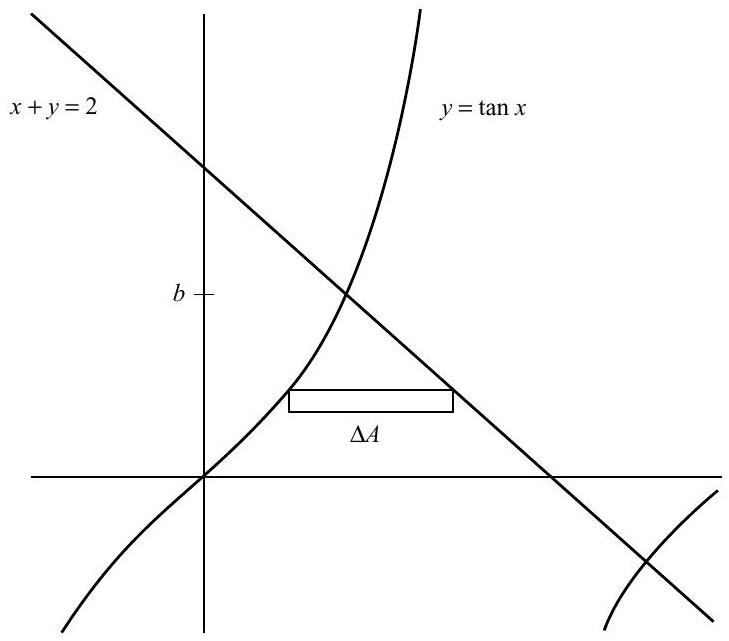
\includegraphics[width=0.40\linewidth]{calculus/images/4dd0024d-5e0f-40f8-af74-ec664288d8ef-31_641_729_301_642.jpg}
\end{center}
\end{solution}

\newpage






\question
An ellipse has major axis 20 and minor axis 10 . Rounded off to the nearest integer, the maximum area of an inscribed rectangle is
\begin{choices}
  \choice $50$
  \choice $79$
  \choice $80$
  \choice $82$
  \CorrectChoice $100$
\end{choices}
\begin{solution}
(E) Center the ellipse at the origin and let $(x, y)$ be the coordinates of the vertex of the inscribed rectangle in the first quadrant, as shown in the figure.\\
\begin{center}
  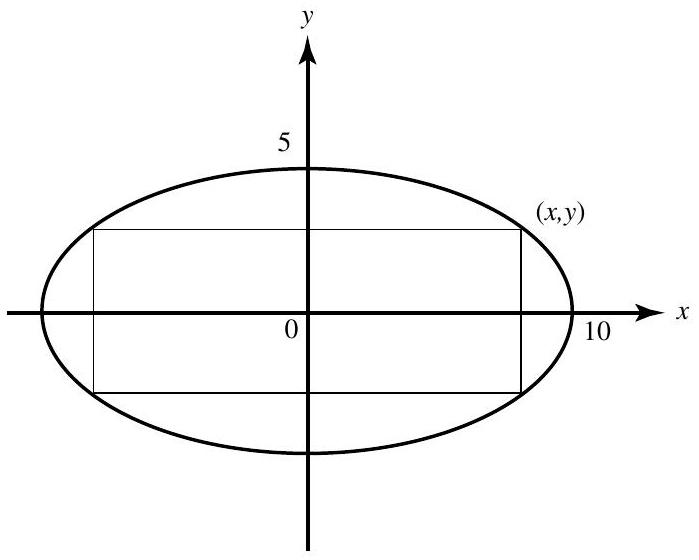
\includegraphics[width=0.40\linewidth]{calculus/images/4dd0024d-5e0f-40f8-af74-ec664288d8ef-31_560_699_1099_691.jpg}
\end{center}
\[
\dfrac{x^{2}}{100}+\dfrac{y^{2}}{25}=1
\]
To maximize the rectangle's area $A=4 x y$, solve the equation of the ellipse, getting
\[
x=\sqrt{100-4 y^{2}}=2 \sqrt{25-y^{2}} .
\]
So $A=8 y \sqrt{25-y^{2}}$. Graph $y=8 x \sqrt{\left(25-x^{2}\right)}$ in the window $[0,5] \times[0,150]$.\\
The calculator shows that the maximum area (the $y$-coordinate) equals 100 .\\
\begin{center}
  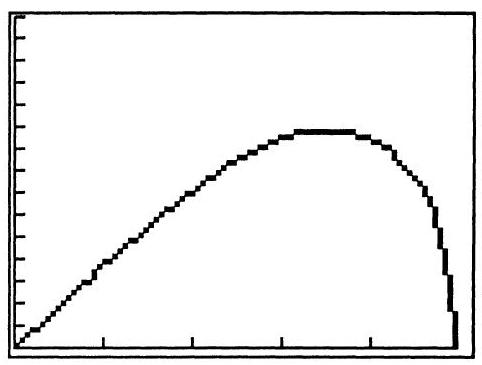
\includegraphics[width=0.40\linewidth]{calculus/images/4dd0024d-5e0f-40f8-af74-ec664288d8ef-31_365_482_2277_797.jpg}
\end{center}
\end{solution}



\newpage



\question
The average value of $y=x \ln x$ on the interval $1 \leqq x \leqq e$ is
\begin{choices}
  \choice $0.772$
  \CorrectChoice $1.221$
  \choice $1.359$
  \choice $1.790$
  \choice $2.097$
\end{choices}
\begin{solution}
(B) $\dfrac{\displaystyle\int_{1}^{e} x \ln x d x}{e-1} \simeq 1.221$.
\end{solution}

\question
Let $f(x)=\displaystyle\int_{0}^{x}\left(1-2 \cos ^{3} t\right) d t$ for $0 \leqq x \leqq 2 \pi$. On which interval is $f$ increasing?
\begin{choices}
  \choice $0<x<\pi$
  \CorrectChoice $0.654<x<5.629$
  \choice $0.654<x<2 \pi$
  \choice $\pi<x<2 \pi$
  \choice none of these
\end{choices}
\begin{solution}
(B) When $f^{\prime}$ is positive, $f$ increases. By the Fundamental Theorem of Calculus, $f^{\prime}(x)=1-2(\cos x)^{3} . \operatorname{Graph} f^{\prime}$ in $[0,2 \pi] \times[-2,4]$. It is clear that $f^{\prime}>0$ on the interval $a<x<b$. Using the calculator to solve $(-2 \cos x)^{3}=0$ yields $a=0.654$ and $b=5.629$.\\
\begin{center}
  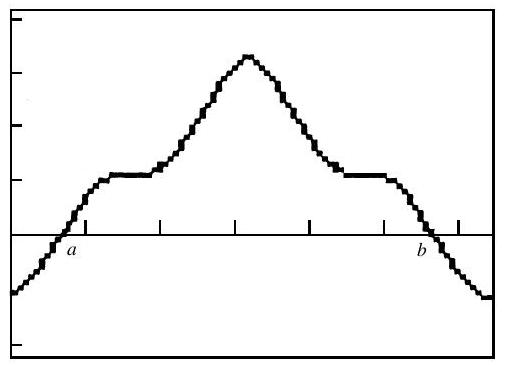
\includegraphics[width=0.40\linewidth]{calculus/images/4dd0024d-5e0f-40f8-af74-ec664288d8ef-32_365_505_709_1159.jpg}
\end{center}
\end{solution}




\newpage






\question
The table shows the speed of an object (in ft/sec) during a 3-sec period. Estimate its acceleration (in $\mathrm{ft} / \mathrm{sec}^{2}$ ) at $t=1.5 \mathrm{sec}$.
\begin{center}
\begin{tabular}{l|r|r|r|r}
time, sec & 0 & 1 & 2 & 3 \\
\hline
speed, ft/sec & 30 & 22 & 12 & 0 \\
\end{tabular}
\end{center}
\begin{choices}
  \choice $-17$
  \choice $-13$
  \CorrectChoice $-10$
  \choice $-5$
  \choice $17$
\end{choices}
\begin{solution}
(C) $a(1.5) \simeq \dfrac{v(2)-v(1)}{2-1}=\dfrac{12-22}{1}$.
\end{solution}






\newpage





\question
A maple-syrup storage tank 16 ft high hangs on a wall. The back is in the shape of the parabola $y=x^{2}$ and all cross sections parallel to the floor are squares. If syrup is pouring in at the rate of $12 \mathrm{ft}^{3} / \mathrm{hr}$, how fast (in $\mathrm{ft} / \mathrm{hr}$ ) is the syrup level rising when it is 9 ft deep?\\
\begin{center}
  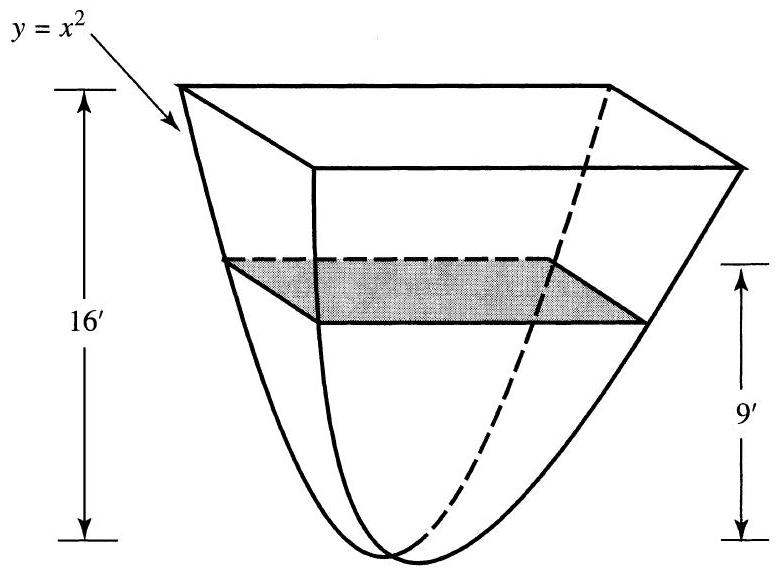
\includegraphics[width=0.40\linewidth]{calculus/images/4dd0024d-5e0f-40f8-af74-ec664288d8ef-13_577_780_521_589.jpg}
\end{center}
\begin{choices}
  \choice $\dfrac{2}{27}$
  \CorrectChoice $\dfrac{1}{3}$
  \choice $\dfrac{4}{3}$
  \choice $36$
  \choice $162$
\end{choices}
\begin{solution}
(B) The volume is composed of elements of the form $\Delta V=(2 x)^{2} \Delta y$. If $h$ is the depth, in feet, then, after $t \mathrm{hr}$,\\
$V(h)=4 \displaystyle\int_{0}^{h} y d y$ and $\dfrac{d V}{d t}=4 h \dfrac{d h}{d t}$.\\
Thus, $12=4$ (9) $\dfrac{d h}{d t}$\\
and $\dfrac{d h}{d t}=\dfrac{1}{3} \mathrm{ft} / \mathrm{hr}$.\\
\begin{center}
  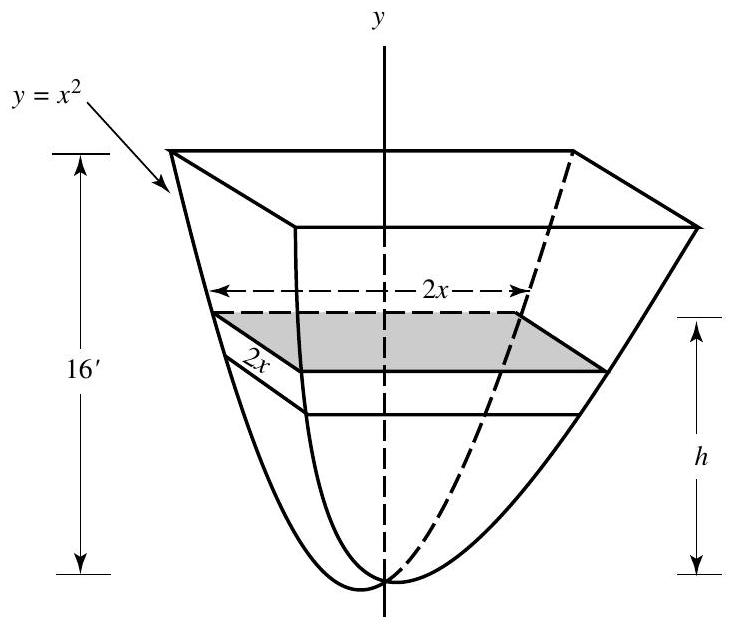
\includegraphics[width=0.40\linewidth]{calculus/images/4dd0024d-5e0f-40f8-af74-ec664288d8ef-32_630_734_1790_1025.jpg}
\end{center}
\end{solution}



\newpage




\question
In a protected area (no predators, no hunters), the deer population increases at a rate of $\dfrac{d P}{d t}=k(1000-P)$, where $P(t)$ represents the population of deer at $t \mathrm{yr}$. If 300 deer were originally placed in the area and a census showed the population had grown to 500 in 5 yr , how many deer will there be after 10 yr ?
\begin{choices}
  \choice $608$
  \CorrectChoice $643$
  \choice $700$
  \choice $833$
  \choice $892$
\end{choices}
\begin{solution}
(B) Separating variables yields

\[
\begin{aligned}
\dfrac{d P}{1000-P} & =k d t, \\
-\ln (1000-P) & =k t+C, \\
1000-P & =c e^{-k t}
\end{aligned}
\]

Then

\[
\begin{gathered}
P(t)=1000-c e^{-k t} \\
P(0)=300 \text { gives } c=700 . P(5)=500 \text { yields } 500=1000-700 e^{-5 k}, \text { so } \\
k \simeq+0.0673 . \text { Now } P(10)=1000-700 e^{-0.673} \simeq 643 .
\end{gathered}
\]


\end{solution}

\question
Shown is the graph of $f(x)=\dfrac{4}{x^{2}+1}$.\\
\begin{center}
  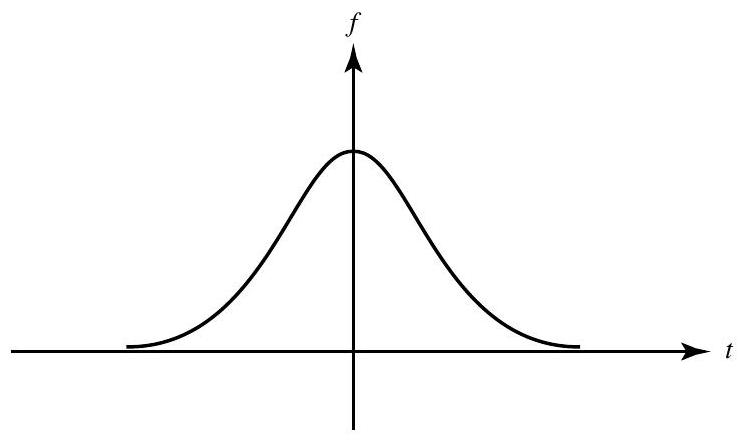
\includegraphics[width=0.40\linewidth]{calculus/images/4dd0024d-5e0f-40f8-af74-ec664288d8ef-13_442_746_1790_607.jpg}
\end{center}

Let $H(x)=\displaystyle\int_{0}^{x} f(t) d t$. The local linearization of $H$ at $x=1$ is $H(x)$ equals
\begin{choices}
  \choice $2 x$
  \choice $-2 x-4$
  \CorrectChoice $2 x+\pi-2$
  \choice $-2 x+\pi+2$
  \choice $2 x+\ln 16+2$
\end{choices}
\begin{solution}
$H(1)=\displaystyle\int_{0}^{1} \dfrac{4}{x^{2}+1} d x=4 \arctan 1=\pi \cdot H^{\prime}(1)=f(1)=2$.
The equation of the tangent line is $y-\pi=2(x-1)$.
\end{solution}



\newpage






\question
A smokestack 100 ft tall is used to treat industrial emissions. The diameters, measured at $25-\mathrm{ft}$ intervals, are shown in the table. Using the midpoint rule, estimate the volume of the smokestack to the nearest $100 \mathrm{ft}^{3}$.\\
\begin{center}
  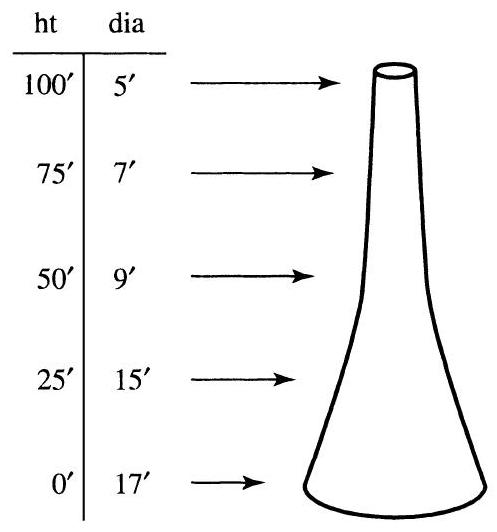
\includegraphics[width=0.40\linewidth]{calculus/images/4dd0024d-5e0f-40f8-af74-ec664288d8ef-14_532_497_494_1106.jpg}
\end{center}
\begin{choices}
  \choice $8100$
  \choice $9500$
  \CorrectChoice $9800$
  \choice $12,500$
  \choice $39,300$
\end{choices}
\begin{solution}
(C) Using midpoint diameters to determine cylinders, estimate the volume to be
\[
V \simeq \pi \cdot 8^{2} \cdot 25+\pi \cdot 6^{2} \cdot 25+\pi \cdot 4^{2} \cdot 25+\pi \cdot 3^{2} \cdot 25
\]
\end{solution}





\newpage




\noindent\textit{In Questions~\ref{calc11:fg-first}--\ref{calc11:fg-last}, the table shows the values of differentiable functions $f$ and $g$.}

\begin{center}
{\renewcommand{\arraystretch}{2.00}
\begin{tabular}{l||r|r||r|r}
$x$ & $f$ & $f^{\prime}$ & $g$ & $g^{\prime}$ \\
\hline
1 & 2 & $\dfrac{1}{2}$ & -3 & 5 \\
\hline
2 & 3 & 1 & 0 & 4 \\
\hline
3 & 4 & 2 & 2 & 3 \\
\hline
4 & 6 & 4 & 3 & $\dfrac{1}{2}$ \\
\hline
\end{tabular}}
\end{center}

\question\label{calc11:fg-first}
If $P(x)=\dfrac{f(x)}{g(x)}$, then $P^{\prime}(3)=$
\begin{choices}
  \CorrectChoice $-2$
  \choice $-\dfrac{8}{9}$
  \choice $-\dfrac{1}{2}$
  \choice $\dfrac{2}{3}$
  \choice $2$
\end{choices}
\begin{solution}
$\left(\dfrac{f}{g}\right)^{\prime}(3)=\dfrac{g(3) \cdot f^{\prime}(3)-f(3) \cdot g^{\prime}(3)}{(g(3))^{2}}=\dfrac{2(2)-4(3)}{2^{2}}$.
\end{solution}

\question
If $H(x)=f(g(x))$, then $H^{\prime}(3)=$
\begin{choices}
  \choice $1$
  \choice $2$
  \CorrectChoice $3$
  \choice $6$
  \choice $9$
\end{choices}
\begin{solution}
$H^{\prime}(3)=f^{\prime}(g(3)) \cdot g^{\prime}(3)=f^{\prime}(2) \cdot g^{\prime}(3)$.
\end{solution}

\question
If $M(x)=f(x) \cdot g(x)$, then $M^{\prime}(3)=$
\begin{choices}
  \choice $2$
  \choice $6$
  \choice $8$
  \choice $14$
  \CorrectChoice $16$
\end{choices}
\begin{solution}
$M^{\prime}(3)=f(3) \cdot g^{\prime}(3)+g(3) \cdot f^{\prime}(3)=4 \cdot 3+2 \cdot 2$.
\end{solution}

\question
If $K(x)=g^{-1}(x)$, then $K^{\prime}(3)=$
\begin{choices}
  \choice $-\dfrac{1}{2}$
  \choice $-\dfrac{1}{3}$
  \choice $\dfrac{1}{3}$
  \choice $\dfrac{1}{2}$
  \choice $2$
\end{choices}
\begin{solution}
$K^{\prime}(3)=\dfrac{1}{g^{\prime}(K(3))}=\dfrac{1}{g^{\prime}\left(g^{-1}(3)\right)}=\dfrac{1}{g^{\prime}(4)}=\dfrac{1}{\dfrac{1}{2}}$.
\end{solution}

\question\label{calc11:fg-last}
If $R(x)=\sqrt{f(x)}$, then $R^{\prime}(3)=$
\begin{choices}
  \choice $\dfrac{1}{4}$
  \choice $\dfrac{1}{2 \sqrt{2}}$
  \choice $\dfrac{1}{2}$
  \choice $\sqrt{2}$
  \choice $2$
\end{choices}
\begin{solution}
$R^{\prime}(3)=\dfrac{1}{2}(f(3))^{-1 / 2} \cdot f^{\prime}(3)$.
\end{solution}




\newpage





\question
Water is poured into a spherical tank at a constant rate. If $W(t)$ is the rate of increase of the depth of the water, then $W$ is
\begin{choices}
  \choice constant
  \choice linear and increasing
  \choice linear and decreasing
  \choice concave up
  \choice concave down
\end{choices}
\begin{solution}
Here are the pertinent curves, with $d$ denoting the depth of the water:\\
\begin{center}
  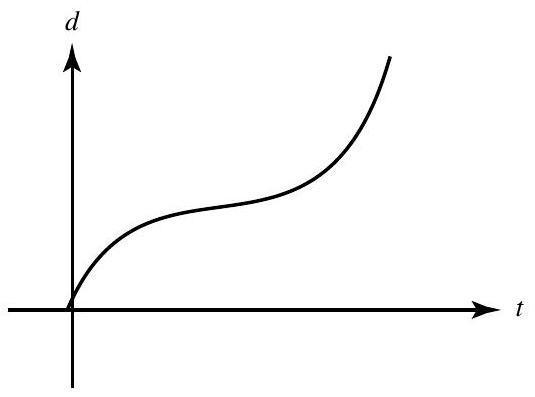
\includegraphics[width=0.40\linewidth]{calculus/images/4dd0024d-5e0f-40f8-af74-ec664288d8ef-33_397_535_2027_463.jpg}
\end{center}
\begin{center}
  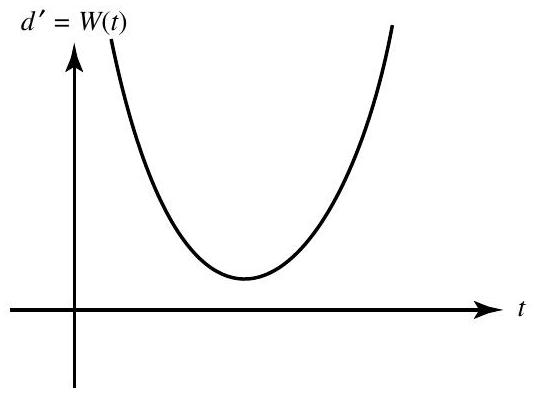
\includegraphics[width=0.40\linewidth]{calculus/images/4dd0024d-5e0f-40f8-af74-ec664288d8ef-33_397_535_2027_1124.jpg}
\end{center}
\end{solution}





\newpage





\question
The graph of $f^{\prime}$ is shown below. If $f(7)=3$ then $f(1)=$\\
\begin{center}
  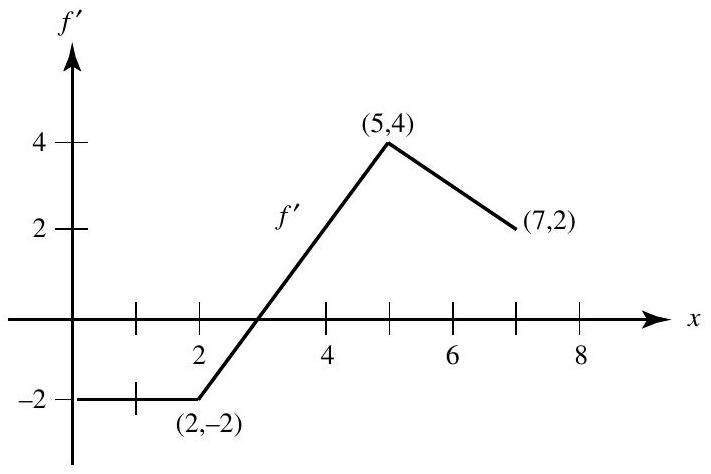
\includegraphics[width=0.40\linewidth]{calculus/images/4dd0024d-5e0f-40f8-af74-ec664288d8ef-15_474_711_886_630.jpg}
\end{center}
\begin{choices}
  \choice $-10$
  \choice $-4$
  \choice $-3$
  \choice $10$
  \choice $16$
\end{choices}
\begin{solution}
Use areas; then $\displaystyle\int_{1}^{7} f^{\prime}=-3+10=7$. Thus, $f(7)-f(1)=7$.
\end{solution}




\newpage


\question
At an outdoor concert, the crowd stands in front of the stage filling a semicircular disk of radius 100 yd . The approximate density of the crowd $x \mathrm{yd}$ from the stage is given by
\[
D(x)=\dfrac{20}{2 \sqrt{x}+1}
\]
people per square yard. About how many people are at the concert?\\
\begin{center}
  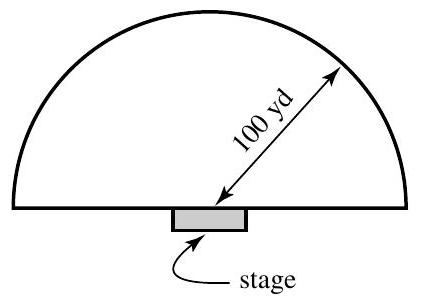
\includegraphics[width=0.40\linewidth]{calculus/images/4dd0024d-5e0f-40f8-af74-ec664288d8ef-15_305_421_1832_774.jpg}
\end{center}
\begin{choices}
  \choice $200$
  \choice $19,500$
  \choice $21,000$
  \choice $165,000$
  \choice $591,000$
\end{choices}
\begin{solution}
The region $x$ units from the stage can be approximated by the semicircular ring shown; its area is then the product of its circumference and its width.\\
\begin{center}
  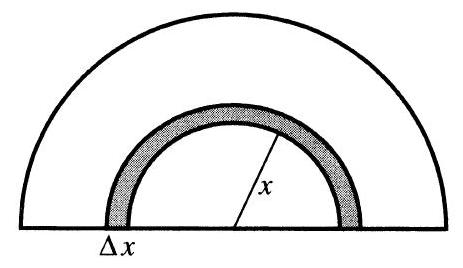
\includegraphics[width=0.40\linewidth]{calculus/images/4dd0024d-5e0f-40f8-af74-ec664288d8ef-34_268_463_431_1145.jpg}
\end{center}
\begin{center}
  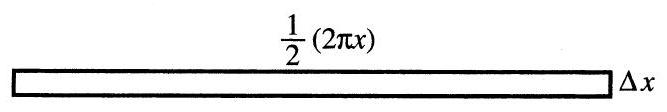
\includegraphics[width=0.40\linewidth]{calculus/images/4dd0024d-5e0f-40f8-af74-ec664288d8ef-34_112_667_784_1066.jpg}
\end{center}
The number of people standing in the region is the product of the area and the density:
\[
\Delta P=(\pi x \Delta x)\left(\dfrac{20}{2 \sqrt{x}+1}\right)
\]
To find the total number of people, evaluate
\[
20 \pi \displaystyle\int_{0}^{100} \dfrac{x}{2 \sqrt{x}+1} d x
\]
\end{solution}



\newpage


\question
The Centers for Disease Control announced that, although more AIDS cases were reported this year, the rate of increase is slowing down. If we graph the number of AIDS cases as a function of time, the curve is currently
\begin{choices}
  \choice increasing and linear
  \choice increasing and concave down
  \choice increasing and concave up
  \choice decreasing and concave down
  \choice decreasing and concave up
\end{choices}
\begin{solution}
$\dfrac{d y}{d t}$ is positive, but decreasing; hence $\dfrac{d y^{2}}{d t^{2}}<0$.
\end{solution}



\newpage




\noindent\textit{In Questions~\ref{calc11:velocity-first}--\ref{calc11:velocity-last}, the graph below shows the velocity, in feet per second, for $0<t<8$, of an object moving along a straight line.}

\begin{center}
  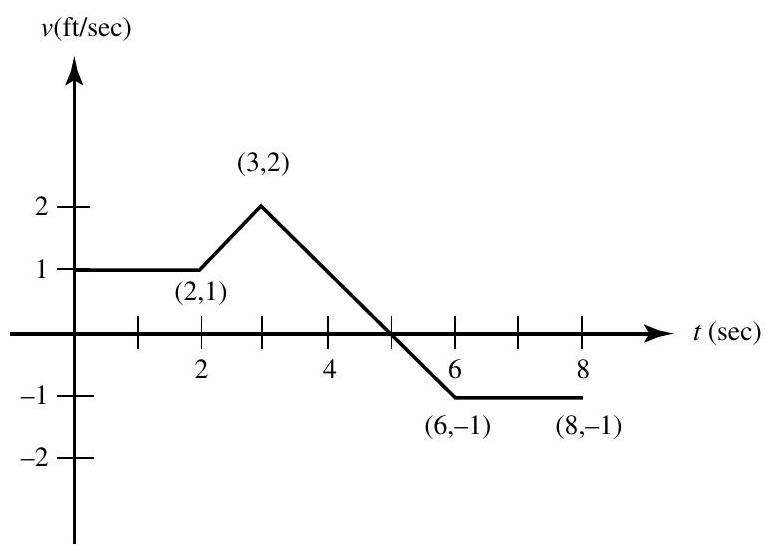
\includegraphics[width=0.40\linewidth]{calculus/images/4dd0024d-5e0f-40f8-af74-ec664288d8ef-16_555_773_422_969.jpg}
\end{center}

\question\label{calc11:velocity-first}
The object's average speed (in $\mathrm{ft} / \mathrm{sec}$ ) for this 8 -sec interval was
\begin{choices}
  \choice $0$
  \choice $\dfrac{3}{8}$
  \choice $1$
  \choice $\dfrac{8}{3}$
  \choice $8$
\end{choices}
\begin{solution}
Average speed $=\dfrac{\text { total distance }}{\text { elapsed time }}=\dfrac{\text { total area }}{8}=\dfrac{8}{8}$.
\end{solution}

\question
When did the object return to the position it occupied at $t=2$ ?
\begin{choices}
  \choice $t=4$
  \choice $t=5$
  \choice $t=6$
  \choice $t=8$
  \choice never
\end{choices}
\begin{solution}
On $2 \leqslant t \leqslant 5$, the object moved $3 \dfrac{1}{2} \mathrm{ft}$ to the right; then on $5 \leqslant t \leqslant 8$, it moved only $2 \dfrac{1}{2} \mathrm{ft}$ to the left.
\end{solution}



\newpage





\question\label{calc11:velocity-last}
The object's average acceleration (in $\mathrm{ft} / \mathrm{sec}^{2}$ ) for this 8 -sec interval was
\begin{choices}
  \choice $-2$
  \choice $-\dfrac{1}{4}$
  \choice $0$
  \choice $\dfrac{1}{4}$
  \choice $1$
\end{choices}
\begin{solution}
Average acceleration $=\dfrac{\Delta v}{\Delta t}=\dfrac{v(8)-v(0)}{8-0}=\dfrac{-1-1}{8}$.
\end{solution}


\newpage





\question
If a block of ice melts at the rate of $\dfrac{72}{2 t+3} \mathrm{~cm}^{3} / \mathrm{min}$, how much ice melts during the first 3 min?
\begin{choices}
  \choice $8 \mathrm{~cm}^{3}$
  \choice $16 \mathrm{~cm}^{3}$
  \choice $21 \mathrm{~cm}^{3}$
  \choice $40 \mathrm{~cm}^{3}$
  \choice $79 \mathrm{~cm}^{3}$
\end{choices}
\begin{solution}
Evaluate $\displaystyle\int_{0}^{3} \dfrac{72}{2 t+3} d t=\left.36 \ln (2 t+3)\right|_{0} ^{3}=36 \ln 3$.
\end{solution}

\question
A particle moves counterclockwise on the circle $x^{2}+y^{2}=25$ with a constant speed of $2 \mathrm{ft} / \mathrm{sec}$. Its velocity vector, $\mathbf{v}$, when the particle is at $(3,4)$, equals
\begin{choices}
  \choice $-\dfrac{1}{5}(8 \mathbf{i}-6 \mathbf{j})$
  \choice $\dfrac{1}{5}(8 \mathbf{i}-6 \mathbf{j})$
  \choice $-2 \sqrt{3} \mathbf{i}+2 \mathbf{j}$
  \choice $2 \mathbf{i}-2 \sqrt{3} \mathbf{j}$
  \choice $-2 \sqrt{2}(\mathbf{i}-\mathbf{j})$
\end{choices}
\begin{solution}
$2 x \dfrac{d x}{d t}+2 y \dfrac{d y}{d t}=0$ and $\dfrac{d y}{d t}=-\dfrac{3}{4} \dfrac{d x}{d t}$ at the point ( 3,4 ).
Use, also, the facts that the speed is given by $|\mathbf{v}|=\sqrt{\left(\dfrac{d x}{d t}\right)^{2}+\left(\dfrac{d y}{d t}\right)^{2}}$ and that the point moves counterclockwise; then $\left(\dfrac{d x}{d t}\right)^{2}+\left(\dfrac{d y}{d t}\right)^{2}=4$, yielding $\dfrac{d x}{d t}=-\dfrac{8}{5}$ and $\dfrac{d y}{d t}=+\dfrac{6}{5}$ at the given point. The velocity vector, $\mathbf{v}$, at ( 3,4 ) must therefore be $-\dfrac{8}{5} \mathbf{i}+\dfrac{6}{5} \mathbf{j}$.
\end{solution}

\question
Let $\mathbf{R}=(a \cos k t) \mathbf{i}+(a \sin k t) \mathbf{j}$ be the (position) vector $x \mathbf{i}+y \mathbf{j}$ from the origin to a moving point $P(x, y)$ at time $t$, where $a$ and $k$ are positive constants. The acceleration vector, $\mathbf{a}$, equals
\begin{choices}
  \choice $-k^{2} \mathbf{R}$
  \choice $a^{2} k^{2} \mathbf{R}$
  \choice $-a \mathbf{R}$
  \choice $-a k^{2}(\cos t \mathbf{i}+\sin t \mathbf{j})$
  \choice $-R$
\end{choices}
\begin{solution}
(A) $\mathbf{v}=-a k \sin k t \mathbf{i}+a k \cos k t \mathbf{j}$, and
\[
\mathbf{a}=-a k^{2} \cos k t \mathbf{i}-a k^{2} \sin k t \mathbf{j}=-k^{2} \mathbf{R} .
\]
\end{solution}





\newpage





\question
The length of the curve $y=2^{x}$ between $(0,1)$ and $(2,4)$ is
\begin{choices}
  \choice $3.141$
  \choice $3.664$
  \choice $4.823$
  \choice $5.000$
  \choice $7.199$
\end{choices}
\begin{solution}
The formula for length of arc is


\[
L=\displaystyle\int_{a}^{b} \sqrt{1+\left(\dfrac{d y}{d x}\right)^{2}} d x
\]

Since $y=2^{x}$, we find

\[
L=\displaystyle\int_{0}^{2} \sqrt{1+\left(2^{x} \ln 2\right)^{2}} d x \simeq 3.664
\]


\end{solution}

\question
The position of a moving object is given by $P(t)=\left(3 t, e^{t}\right)$. Its acceleration is
\begin{choices}
  \choice undefined
  \choice constant in both magnitude and direction
  \choice constant in magnitude only
  \choice constant in direction only
  \choice constant in neither magnitude nor direction
\end{choices}
\begin{solution}
$\mathbf{a}(t)=\left(0, e^{t}\right)$; the acceleration is always upward.
\end{solution}

\question
Suppose we plot a particular solution of $\dfrac{d y}{d x}=4 y$ from initial point $(0,1)$ using Euler's method. After one step of size $\Delta x=0.1$, how big is the error?
\begin{choices}
  \choice $0.09$
  \choice $1.09$
  \choice $1.49$
  \choice $1.90$
  \choice $2.65$
\end{choices}
\begin{solution}
At $(0,1), \dfrac{d y}{d x}=4$, so Euler's method yields $(0.1,1+0.1(4))=(0.1,1.4)$.
\[
\dfrac{d y}{d x}=4 y \text { has particular solution } y=e^{4 x} ; \text { the error is } e^{4(0.1)}-1.4 .
\]
\end{solution}




\newpage



\question
We use the first three terms to estimate $\sum\limits_{n=0}^{\infty} \dfrac{(-1)^{n}}{n^{2}+1}$. Which of the following statements is (are) true?

\statementbox{%
\begin{enumerate}
\renewcommand{\labelenumi}{\Roman{enumi}.}
\item The estimate is 0.7.
\item The estimate is too low.
\item The estimate is off by less than 0.1.
\end{enumerate}%
}
\begin{choices}
  \choice I only
  \choice III only
  \choice I and II
  \choice I and III
  \choice all three
\end{choices}
\begin{solution}
$1-\dfrac{1}{2}+\dfrac{1}{5}=0.7$. Note that the series converges by the Alternating Series


Test. Since the first term dropped in the estimate is $-\dfrac{1}{10}$, the estimate is too high, but within 0.1 of the true sum.
\end{solution}

\question
Which of these diverges?
\begin{choices}
  \choice $\sum\limits_{n=1}^{\infty} \dfrac{2}{3^{n}}$
  \choice $\sum\limits_{n=1}^{\infty}\left(\dfrac{2}{3}\right)^{n}$
  \choice $\sum\limits_{n=1}^{\infty} \dfrac{2}{3 n}$
  \choice $\sum\limits_{n=1}^{\infty} \dfrac{2}{n^{3}}$
  \choice $\sum\limits_{n=1}^{\infty} \dfrac{2 n}{3^{n}}$
\end{choices}
\begin{solution}
(C) $\sum\limits_{n=1}^{\infty} \dfrac{2}{3 n}=\dfrac{2}{3} \sum\limits_{n=1}^{\infty} \dfrac{1}{n}$, which equals a constant times the harmonic series.
\end{solution}





\newpage





\question
Find the radius of convergence of $\sum\limits_{n=1}^{\infty} \dfrac{n!}{n^{n}} x^{n}$.
\begin{choices}
  \choice $0$
  \choice $\dfrac{1}{e}$
  \choice $1$
  \choice $e$
  \choice $\infty$
\end{choices}
\begin{solution}
(D) We seek $x$ such that

\[
\lim\limits_{n \to \infty}\left|\dfrac{(n+1)!\cdot x^{n+1}}{(n+1)^{n+1}} \cdot \dfrac{n^{n}}{n!\cdot x^{n}}\right|<1
\]

or such that $|x| \cdot \lim\limits_{n \to \infty}\left(\dfrac{n}{n+1}\right)^{n}<1$\\
or such that $|x|<\dfrac{1}{\lim\limits_{n \to \infty}\left(\dfrac{n}{n+1}\right)^{n}}$.\\
The fraction equals $\lim\limits_{n \to \infty}\left(\dfrac{n+1}{n}\right)^{n} \lim\limits_{n \to \infty}\left(1+\dfrac{1}{n}\right)^{n}=e$.\\
Then $|x|<e$ and the radius of convergence is $e$.
\end{solution}

\question
When we use $e^{x} \simeq 1+x+\dfrac{x^{2}}{2}$ to estimate $\sqrt{e}$, the Lagrange remainder is no greater than
\begin{choices}
  \choice $0.021$
  \choice $0.034$
  \choice $0.042$
  \choice $0.067$
  \choice $0.742$
\end{choices}
\begin{solution}
(B) The error is less than the maximum value of $\dfrac{e^{c}}{3!} x^{3}$ for $0 \leq x \leq \dfrac{1}{2}$.\\
This maximum occurs at $c=x=\dfrac{1}{2}$.
\end{solution}





\newpage






\question
An object in motion along a curve has position $P(t)=(\tan t, \cos 2 t)$ for $0 \leqslant t \leqslant 1$. How far does it travel?
\begin{choices}
  \choice $0.96$
  \choice $1.73$
  \choice $2.10$
  \choice $2.14$
  \choice $3.98$
\end{choices}
\begin{solution}
(D) Distance $=\displaystyle\int_{0}^{1} \sqrt{\left(\dfrac{d x}{d t}\right)^{2}+\left(\dfrac{d y}{d t}\right)^{2}} d t$.

\[
=\displaystyle\int_{0}^{1} \sqrt{\left(\sec ^{2} t\right)^{2}+(-2 \sin 2 t)^{2}} d t
\]

Note that the curve is traced exactly once by the parametric equations from $t=0$ to $t=1$.
\end{solution}